\documentclass[twoside]{book}

% Packages required by doxygen
\usepackage{fixltx2e}
\usepackage{calc}
\usepackage{doxygen}
\usepackage[export]{adjustbox} % also loads graphicx
\usepackage{graphicx}
\usepackage[utf8]{inputenc}
\usepackage{makeidx}
\usepackage{multicol}
\usepackage{multirow}
\PassOptionsToPackage{warn}{textcomp}
\usepackage{textcomp}
\usepackage[nointegrals]{wasysym}
\usepackage[table]{xcolor}

% Font selection
\usepackage[T1]{fontenc}
\usepackage[scaled=.90]{helvet}
\usepackage{courier}
\usepackage{amssymb}
\usepackage{sectsty}
\renewcommand{\familydefault}{\sfdefault}
\allsectionsfont{%
  \fontseries{bc}\selectfont%
  \color{darkgray}%
}
\renewcommand{\DoxyLabelFont}{%
  \fontseries{bc}\selectfont%
  \color{darkgray}%
}
\newcommand{\+}{\discretionary{\mbox{\scriptsize$\hookleftarrow$}}{}{}}

% Page & text layout
\usepackage{geometry}
\geometry{%
  a4paper,%
  top=2.5cm,%
  bottom=2.5cm,%
  left=2.5cm,%
  right=2.5cm%
}
\tolerance=750
\hfuzz=15pt
\hbadness=750
\setlength{\emergencystretch}{15pt}
\setlength{\parindent}{0cm}
\setlength{\parskip}{3ex plus 2ex minus 2ex}
\makeatletter
\renewcommand{\paragraph}{%
  \@startsection{paragraph}{4}{0ex}{-1.0ex}{1.0ex}{%
    \normalfont\normalsize\bfseries\SS@parafont%
  }%
}
\renewcommand{\subparagraph}{%
  \@startsection{subparagraph}{5}{0ex}{-1.0ex}{1.0ex}{%
    \normalfont\normalsize\bfseries\SS@subparafont%
  }%
}
\makeatother

% Headers & footers
\usepackage{fancyhdr}
\pagestyle{fancyplain}
\fancyhead[LE]{\fancyplain{}{\bfseries\thepage}}
\fancyhead[CE]{\fancyplain{}{}}
\fancyhead[RE]{\fancyplain{}{\bfseries\leftmark}}
\fancyhead[LO]{\fancyplain{}{\bfseries\rightmark}}
\fancyhead[CO]{\fancyplain{}{}}
\fancyhead[RO]{\fancyplain{}{\bfseries\thepage}}
\fancyfoot[LE]{\fancyplain{}{}}
\fancyfoot[CE]{\fancyplain{}{}}
\fancyfoot[RE]{\fancyplain{}{\bfseries\scriptsize Generated by Doxygen }}
\fancyfoot[LO]{\fancyplain{}{\bfseries\scriptsize Generated by Doxygen }}
\fancyfoot[CO]{\fancyplain{}{}}
\fancyfoot[RO]{\fancyplain{}{}}
\renewcommand{\footrulewidth}{0.4pt}
\renewcommand{\chaptermark}[1]{%
  \markboth{#1}{}%
}
\renewcommand{\sectionmark}[1]{%
  \markright{\thesection\ #1}%
}

% Indices & bibliography
\usepackage{natbib}
\usepackage[titles]{tocloft}
\setcounter{tocdepth}{3}
\setcounter{secnumdepth}{5}
\makeindex

% Custom commands
\newcommand{\clearemptydoublepage}{%
  \newpage{\pagestyle{empty}\cleardoublepage}%
}

\usepackage{caption}
\captionsetup{labelsep=space,justification=centering,font={bf},singlelinecheck=off,skip=4pt,position=top}

%===== C O N T E N T S =====

\begin{document}

% Titlepage & ToC
\pagenumbering{alph}
\begin{titlepage}
\vspace*{7cm}
\begin{center}%
{\Large Ceneo\+HD }\\
\vspace*{1cm}
{\large Generated by Doxygen 1.8.14}\\
\end{center}
\end{titlepage}
\clearemptydoublepage
\pagenumbering{roman}
\tableofcontents
\clearemptydoublepage
\pagenumbering{arabic}

%--- Begin generated contents ---
\chapter{Hierarchical Index}
\section{Class Hierarchy}
This inheritance list is sorted roughly, but not completely, alphabetically\+:\begin{DoxyCompactList}
\item \contentsline{section}{com.\+project.\+application.\+Ceneo\+H\+D\+Component}{\pageref{classcom_1_1project_1_1application_1_1_ceneo_h_d_component}}{}
\item Exception\begin{DoxyCompactList}
\item \contentsline{section}{com.\+project.\+base.\+Provider\+Exception}{\pageref{classcom_1_1project_1_1base_1_1_provider_exception}}{}
\end{DoxyCompactList}
\item \contentsline{section}{com.\+project.\+application.\+Export\+Reviews\+Argument}{\pageref{classcom_1_1project_1_1application_1_1_export_reviews_argument}}{}
\item \contentsline{section}{com.\+project.\+application.\+Export\+Reviews\+Format}{\pageref{enumcom_1_1project_1_1application_1_1_export_reviews_format}}{}
\item \contentsline{section}{com.\+project.\+base.\+On\+Error\+Listener}{\pageref{interfacecom_1_1project_1_1base_1_1_on_error_listener}}{}
\item \contentsline{section}{com.\+project.\+base.\+On\+Success\+Listener$<$ R\+E\+S\+U\+L\+T\+\_\+\+O\+B\+J\+E\+CT $>$}{\pageref{interfacecom_1_1project_1_1base_1_1_on_success_listener}}{}
\item \contentsline{section}{com.\+project.\+dto.\+Product\+D\+TO}{\pageref{classcom_1_1project_1_1dto_1_1_product_d_t_o}}{}
\item \contentsline{section}{com.\+project.\+entity.\+Product\+Entity}{\pageref{classcom_1_1project_1_1entity_1_1_product_entity}}{}
\item \contentsline{section}{com.\+project.\+dto.\+Product\+Reviews\+D\+TO}{\pageref{classcom_1_1project_1_1dto_1_1_product_reviews_d_t_o}}{}
\item \contentsline{section}{com.\+project.\+dto.\+Review\+D\+TO}{\pageref{classcom_1_1project_1_1dto_1_1_review_d_t_o}}{}
\item \contentsline{section}{com.\+project.\+entity.\+Review\+Entity}{\pageref{classcom_1_1project_1_1entity_1_1_review_entity}}{}
\item Runtime\+Exception\begin{DoxyCompactList}
\item \contentsline{section}{com.\+project.\+base.\+Database\+Exception}{\pageref{classcom_1_1project_1_1base_1_1_database_exception}}{}
\end{DoxyCompactList}
\item \contentsline{section}{com.\+project.\+base.\+Use\+Case$<$ R\+E\+Q\+U\+E\+S\+T\+\_\+\+O\+B\+J\+E\+CT, R\+E\+S\+P\+O\+N\+S\+E\+\_\+\+O\+B\+J\+E\+CT $>$}{\pageref{interfacecom_1_1project_1_1base_1_1_use_case}}{}
\item \contentsline{section}{com.\+project.\+base.\+Use\+Case$<$ com.\+project.\+dto.\+Product\+Reviews\+D\+TO, com.\+project.\+entity.\+Product\+Entity $>$}{\pageref{interfacecom_1_1project_1_1base_1_1_use_case}}{}
\item \contentsline{section}{com.\+project.\+base.\+Use\+Case$<$ com.\+project.\+entity.\+Product\+Entity, Void $>$}{\pageref{interfacecom_1_1project_1_1base_1_1_use_case}}{}
\item \contentsline{section}{com.\+project.\+base.\+Use\+Case$<$ Export\+Reviews\+Argument, File $>$}{\pageref{interfacecom_1_1project_1_1base_1_1_use_case}}{}
\item \contentsline{section}{com.\+project.\+base.\+Use\+Case$<$ Product\+Entity, Void $>$}{\pageref{interfacecom_1_1project_1_1base_1_1_use_case}}{}
\item \contentsline{section}{com.\+project.\+base.\+Use\+Case$<$ Product\+Reviews\+D\+TO, Product\+Entity $>$}{\pageref{interfacecom_1_1project_1_1base_1_1_use_case}}{}
\item \contentsline{section}{com.\+project.\+base.\+Use\+Case$<$ String, com.\+project.\+dto.\+Product\+Reviews\+D\+TO $>$}{\pageref{interfacecom_1_1project_1_1base_1_1_use_case}}{}
\item \contentsline{section}{com.\+project.\+base.\+Use\+Case$<$ String, List$<$ Product\+D\+TO $>$ $>$}{\pageref{interfacecom_1_1project_1_1base_1_1_use_case}}{}
\item \contentsline{section}{com.\+project.\+base.\+Use\+Case$<$ String, List$<$ Review\+Entity $>$ $>$}{\pageref{interfacecom_1_1project_1_1base_1_1_use_case}}{}
\item \contentsline{section}{com.\+project.\+base.\+Use\+Case$<$ String, Product\+Reviews\+D\+TO $>$}{\pageref{interfacecom_1_1project_1_1base_1_1_use_case}}{}
\item \contentsline{section}{com.\+project.\+base.\+Use\+Case$<$ String, Void $>$}{\pageref{interfacecom_1_1project_1_1base_1_1_use_case}}{}
\item \contentsline{section}{com.\+project.\+base.\+Use\+Case$<$ Void, List$<$ Product\+Entity $>$ $>$}{\pageref{interfacecom_1_1project_1_1base_1_1_use_case}}{}
\item \contentsline{section}{com.\+project.\+base.\+Use\+Case$<$ Void, Void $>$}{\pageref{interfacecom_1_1project_1_1base_1_1_use_case}}{}
\item \contentsline{section}{com.\+project.\+base.\+Use\+Case\+Executor}{\pageref{interfacecom_1_1project_1_1base_1_1_use_case_executor}}{}
\end{DoxyCompactList}

\chapter{Class Index}
\section{Class List}
Here are the classes, structs, unions and interfaces with brief descriptions\+:\begin{DoxyCompactList}
\item\contentsline{section}{\textbf{ com.\+project.\+application.\+Ceneo\+H\+D\+Component} }{\pageref{classcom_1_1project_1_1application_1_1_ceneo_h_d_component}}{}
\item\contentsline{section}{\textbf{ com.\+project.\+base.\+Database\+Exception} }{\pageref{classcom_1_1project_1_1base_1_1_database_exception}}{}
\item\contentsline{section}{\textbf{ com.\+project.\+application.\+Export\+Reviews\+Argument} }{\pageref{classcom_1_1project_1_1application_1_1_export_reviews_argument}}{}
\item\contentsline{section}{\textbf{ com.\+project.\+application.\+Export\+Reviews\+Format} }{\pageref{enumcom_1_1project_1_1application_1_1_export_reviews_format}}{}
\item\contentsline{section}{\textbf{ com.\+project.\+base.\+On\+Error\+Listener} }{\pageref{interfacecom_1_1project_1_1base_1_1_on_error_listener}}{}
\item\contentsline{section}{\textbf{ com.\+project.\+base.\+On\+Success\+Listener$<$ R\+E\+S\+U\+L\+T\+\_\+\+O\+B\+J\+E\+C\+T $>$} }{\pageref{interfacecom_1_1project_1_1base_1_1_on_success_listener}}{}
\item\contentsline{section}{\textbf{ com.\+project.\+dto.\+Product\+D\+TO} }{\pageref{classcom_1_1project_1_1dto_1_1_product_d_t_o}}{}
\item\contentsline{section}{\textbf{ com.\+project.\+entity.\+Product\+Entity} }{\pageref{classcom_1_1project_1_1entity_1_1_product_entity}}{}
\item\contentsline{section}{\textbf{ com.\+project.\+dto.\+Product\+Reviews\+D\+TO} }{\pageref{classcom_1_1project_1_1dto_1_1_product_reviews_d_t_o}}{}
\item\contentsline{section}{\textbf{ com.\+project.\+base.\+Provider\+Exception} }{\pageref{classcom_1_1project_1_1base_1_1_provider_exception}}{}
\item\contentsline{section}{\textbf{ com.\+project.\+dto.\+Review\+D\+TO} }{\pageref{classcom_1_1project_1_1dto_1_1_review_d_t_o}}{}
\item\contentsline{section}{\textbf{ com.\+project.\+entity.\+Review\+Entity} }{\pageref{classcom_1_1project_1_1entity_1_1_review_entity}}{}
\item\contentsline{section}{\textbf{ com.\+project.\+base.\+Use\+Case$<$ R\+E\+Q\+U\+E\+S\+T\+\_\+\+O\+B\+J\+E\+C\+T, R\+E\+S\+P\+O\+N\+S\+E\+\_\+\+O\+B\+J\+E\+C\+T $>$} }{\pageref{interfacecom_1_1project_1_1base_1_1_use_case}}{}
\item\contentsline{section}{\textbf{ com.\+project.\+base.\+Use\+Case\+Executor} }{\pageref{interfacecom_1_1project_1_1base_1_1_use_case_executor}}{}
\end{DoxyCompactList}

\chapter{Class Documentation}
\section{com.\+project.\+application.\+Ceneo\+H\+D\+Component Class Reference}
\label{classcom_1_1project_1_1application_1_1_ceneo_h_d_component}\index{com.\+project.\+application.\+Ceneo\+H\+D\+Component@{com.\+project.\+application.\+Ceneo\+H\+D\+Component}}
\subsection*{Public Member Functions}
\begin{DoxyCompactItemize}
\item 
\textbf{ Ceneo\+H\+D\+Component} ()
\item 
\textbf{ Use\+Case\+Executor} \textbf{ provide\+Use\+Case\+Executor} ()
\item 
final \textbf{ Use\+Case}$<$ Void, Void $>$ \textbf{ provide\+Initialize\+Application\+Use\+Case} ()
\item 
final \textbf{ Use\+Case}$<$ String, \textbf{ Product\+Reviews\+D\+TO} $>$ \textbf{ provide\+Extract\+Product\+Use\+Case} ()
\item 
final \textbf{ Use\+Case}$<$ \textbf{ Product\+Entity}, Void $>$ \textbf{ provide\+Save\+Product\+Use\+Case} ()
\item 
final \textbf{ Use\+Case}$<$ \textbf{ Product\+Reviews\+D\+TO}, \textbf{ Product\+Entity} $>$ \textbf{ provide\+Transform\+Product\+Use\+Case} ()
\item 
final \textbf{ Use\+Case}$<$ Void, List$<$ \textbf{ Product\+Entity} $>$ $>$ \textbf{ provide\+Load\+Products\+Use\+Case} ()
\item 
final \textbf{ Use\+Case}$<$ \textbf{ Export\+Reviews\+Argument}, File $>$ \textbf{ provide\+Export\+Reviews\+Use\+Case} ()
\item 
final \textbf{ Use\+Case}$<$ Void, Void $>$ \textbf{ provide\+Clear\+Database\+Use\+Case} ()
\item 
final \textbf{ Use\+Case}$<$ String, List$<$ \textbf{ Review\+Entity} $>$ $>$ \textbf{ provide\+Load\+Reviews\+Use\+Case} ()
\item 
final \textbf{ Use\+Case}$<$ String, List$<$ \textbf{ Product\+D\+TO} $>$ $>$ \textbf{ provide\+Search\+Products\+Use\+Case} ()
\item 
final \textbf{ Use\+Case}$<$ String, Void $>$ \textbf{ provide\+E\+T\+L\+Product\+Use\+Case} ()
\end{DoxyCompactItemize}


\subsection{Detailed Description}
\begin{DoxyAuthor}{Author}
seweryn
\end{DoxyAuthor}
Główny komponent aplikacji. Odgrywa rolę kontynera do wstrzykiwania zależności oraz udostępnia usługi. Po stworzeniu instancji należy wykonać usecase inicjalizujący a następnie można pobierać pozostałe komponenty aplikacji. W przeciwnym razie zostanie zgłoszony Runtime\+Exception. 

\subsection{Constructor \& Destructor Documentation}
\mbox{\label{classcom_1_1project_1_1application_1_1_ceneo_h_d_component_a032ecd41ce2b6351994e73b6b67cd87e}} 
\index{com\+::project\+::application\+::\+Ceneo\+H\+D\+Component@{com\+::project\+::application\+::\+Ceneo\+H\+D\+Component}!Ceneo\+H\+D\+Component@{Ceneo\+H\+D\+Component}}
\index{Ceneo\+H\+D\+Component@{Ceneo\+H\+D\+Component}!com\+::project\+::application\+::\+Ceneo\+H\+D\+Component@{com\+::project\+::application\+::\+Ceneo\+H\+D\+Component}}
\subsubsection{Ceneo\+H\+D\+Component()}
{\footnotesize\ttfamily com.\+project.\+application.\+Ceneo\+H\+D\+Component.\+Ceneo\+H\+D\+Component (\begin{DoxyParamCaption}{ }\end{DoxyParamCaption})}

Konstruktor domyślny 

\subsection{Member Function Documentation}
\mbox{\label{classcom_1_1project_1_1application_1_1_ceneo_h_d_component_a6b004c2a137ab6a1f5fb9e869b0d6e30}} 
\index{com\+::project\+::application\+::\+Ceneo\+H\+D\+Component@{com\+::project\+::application\+::\+Ceneo\+H\+D\+Component}!provide\+Clear\+Database\+Use\+Case@{provide\+Clear\+Database\+Use\+Case}}
\index{provide\+Clear\+Database\+Use\+Case@{provide\+Clear\+Database\+Use\+Case}!com\+::project\+::application\+::\+Ceneo\+H\+D\+Component@{com\+::project\+::application\+::\+Ceneo\+H\+D\+Component}}
\subsubsection{provide\+Clear\+Database\+Use\+Case()}
{\footnotesize\ttfamily final \textbf{ Use\+Case}$<$Void,Void$>$ com.\+project.\+application.\+Ceneo\+H\+D\+Component.\+provide\+Clear\+Database\+Use\+Case (\begin{DoxyParamCaption}{ }\end{DoxyParamCaption})}

\begin{DoxyReturn}{Returns}
Clear\+Database\+Use\+Case, który czyści wszystkie tabele bazy danych.
\end{DoxyReturn}
R\+E\+Q\+U\+E\+S\+T\+\_\+\+O\+B\+J\+E\+CT null R\+E\+S\+P\+O\+N\+S\+E\+\_\+\+O\+B\+J\+E\+CT null \mbox{\label{classcom_1_1project_1_1application_1_1_ceneo_h_d_component_a40c80dbc42262aab12e5bd240543657e}} 
\index{com\+::project\+::application\+::\+Ceneo\+H\+D\+Component@{com\+::project\+::application\+::\+Ceneo\+H\+D\+Component}!provide\+E\+T\+L\+Product\+Use\+Case@{provide\+E\+T\+L\+Product\+Use\+Case}}
\index{provide\+E\+T\+L\+Product\+Use\+Case@{provide\+E\+T\+L\+Product\+Use\+Case}!com\+::project\+::application\+::\+Ceneo\+H\+D\+Component@{com\+::project\+::application\+::\+Ceneo\+H\+D\+Component}}
\subsubsection{provide\+E\+T\+L\+Product\+Use\+Case()}
{\footnotesize\ttfamily final \textbf{ Use\+Case}$<$String,Void$>$ com.\+project.\+application.\+Ceneo\+H\+D\+Component.\+provide\+E\+T\+L\+Product\+Use\+Case (\begin{DoxyParamCaption}{ }\end{DoxyParamCaption})}

\begin{DoxyReturn}{Returns}
E\+T\+L\+Product\+Use\+Case, który pozwala na przeprowadzenie całego procesu E\+TL. Pobiera opinie na podstawie product\+\_\+id, przekształca je na ancje a następnie zapisuje do bazy danych.
\end{DoxyReturn}
R\+E\+Q\+U\+E\+S\+T\+\_\+\+O\+B\+J\+E\+CT String -\/ product\+\_\+id R\+E\+S\+P\+O\+N\+S\+E\+\_\+\+O\+B\+J\+E\+CT null \mbox{\label{classcom_1_1project_1_1application_1_1_ceneo_h_d_component_a8a711c9239e375461a2c854aa88bbaa6}} 
\index{com\+::project\+::application\+::\+Ceneo\+H\+D\+Component@{com\+::project\+::application\+::\+Ceneo\+H\+D\+Component}!provide\+Export\+Reviews\+Use\+Case@{provide\+Export\+Reviews\+Use\+Case}}
\index{provide\+Export\+Reviews\+Use\+Case@{provide\+Export\+Reviews\+Use\+Case}!com\+::project\+::application\+::\+Ceneo\+H\+D\+Component@{com\+::project\+::application\+::\+Ceneo\+H\+D\+Component}}
\subsubsection{provide\+Export\+Reviews\+Use\+Case()}
{\footnotesize\ttfamily final \textbf{ Use\+Case}$<$\textbf{ Export\+Reviews\+Argument}, File$>$ com.\+project.\+application.\+Ceneo\+H\+D\+Component.\+provide\+Export\+Reviews\+Use\+Case (\begin{DoxyParamCaption}{ }\end{DoxyParamCaption})}

\begin{DoxyReturn}{Returns}
Export\+Reviews\+Use\+Case, który może zostać użyty do wyeksportowania opini produktu do pliku C\+SV lub plików T\+XT.
\end{DoxyReturn}
R\+E\+Q\+U\+E\+S\+T\+\_\+\+O\+B\+J\+E\+CT \doxyref{Export\+Reviews\+Argument}{p.}{classcom_1_1project_1_1application_1_1_export_reviews_argument} -\/ zawiera konfiguracje eksportu R\+E\+S\+P\+O\+N\+S\+E\+\_\+\+O\+B\+J\+E\+CT File -\/ stworzony plik lub folder \mbox{\label{classcom_1_1project_1_1application_1_1_ceneo_h_d_component_a6f75b50aae33d90a90bfeacc2c6034c0}} 
\index{com\+::project\+::application\+::\+Ceneo\+H\+D\+Component@{com\+::project\+::application\+::\+Ceneo\+H\+D\+Component}!provide\+Extract\+Product\+Use\+Case@{provide\+Extract\+Product\+Use\+Case}}
\index{provide\+Extract\+Product\+Use\+Case@{provide\+Extract\+Product\+Use\+Case}!com\+::project\+::application\+::\+Ceneo\+H\+D\+Component@{com\+::project\+::application\+::\+Ceneo\+H\+D\+Component}}
\subsubsection{provide\+Extract\+Product\+Use\+Case()}
{\footnotesize\ttfamily final \textbf{ Use\+Case}$<$String,\textbf{ Product\+Reviews\+D\+TO}$>$ com.\+project.\+application.\+Ceneo\+H\+D\+Component.\+provide\+Extract\+Product\+Use\+Case (\begin{DoxyParamCaption}{ }\end{DoxyParamCaption})}

\begin{DoxyReturn}{Returns}
Extract\+Product\+Use\+Case, który przeprowadza operacje pobierania opini produktu na podstawie product\+\_\+id.
\end{DoxyReturn}
R\+E\+Q\+U\+E\+S\+T\+\_\+\+O\+B\+J\+E\+CT String -\/ id produktu R\+E\+S\+P\+O\+N\+S\+E\+\_\+\+O\+B\+J\+E\+CT Product\+Reviews\+D\+TO -\/ dane produktu oraz lista opini \mbox{\label{classcom_1_1project_1_1application_1_1_ceneo_h_d_component_ac9ab1ca6002708c209133ad2d5fef869}} 
\index{com\+::project\+::application\+::\+Ceneo\+H\+D\+Component@{com\+::project\+::application\+::\+Ceneo\+H\+D\+Component}!provide\+Initialize\+Application\+Use\+Case@{provide\+Initialize\+Application\+Use\+Case}}
\index{provide\+Initialize\+Application\+Use\+Case@{provide\+Initialize\+Application\+Use\+Case}!com\+::project\+::application\+::\+Ceneo\+H\+D\+Component@{com\+::project\+::application\+::\+Ceneo\+H\+D\+Component}}
\subsubsection{provide\+Initialize\+Application\+Use\+Case()}
{\footnotesize\ttfamily final \textbf{ Use\+Case}$<$Void, Void$>$ com.\+project.\+application.\+Ceneo\+H\+D\+Component.\+provide\+Initialize\+Application\+Use\+Case (\begin{DoxyParamCaption}{ }\end{DoxyParamCaption})}

\begin{DoxyReturn}{Returns}
Initialize\+Application\+Use\+Case odpowiedzialny za inicjalizacje aplikacji, który powinien zostać wykonany zaraz po stworzeniu komponentu \doxyref{Ceneo\+H\+D\+Component}{p.}{classcom_1_1project_1_1application_1_1_ceneo_h_d_component}, przed pobraniem innych komponentów. Po wywołaniu zostanie stworzona baza danych i nawiązane z nią połączenie.
\end{DoxyReturn}
R\+E\+Q\+U\+E\+S\+T\+\_\+\+O\+B\+J\+E\+CT null R\+E\+S\+P\+O\+N\+S\+E\+\_\+\+O\+B\+J\+E\+CT null \mbox{\label{classcom_1_1project_1_1application_1_1_ceneo_h_d_component_ad43cdd2d0c4c4708d6ef2630d9541194}} 
\index{com\+::project\+::application\+::\+Ceneo\+H\+D\+Component@{com\+::project\+::application\+::\+Ceneo\+H\+D\+Component}!provide\+Load\+Products\+Use\+Case@{provide\+Load\+Products\+Use\+Case}}
\index{provide\+Load\+Products\+Use\+Case@{provide\+Load\+Products\+Use\+Case}!com\+::project\+::application\+::\+Ceneo\+H\+D\+Component@{com\+::project\+::application\+::\+Ceneo\+H\+D\+Component}}
\subsubsection{provide\+Load\+Products\+Use\+Case()}
{\footnotesize\ttfamily final \textbf{ Use\+Case}$<$Void,List$<$\textbf{ Product\+Entity}$>$ $>$ com.\+project.\+application.\+Ceneo\+H\+D\+Component.\+provide\+Load\+Products\+Use\+Case (\begin{DoxyParamCaption}{ }\end{DoxyParamCaption})}

\begin{DoxyReturn}{Returns}
Load\+Products\+Use\+Case, który pobiera z bazy danych listę produktów.
\end{DoxyReturn}
R\+E\+Q\+U\+E\+S\+T\+\_\+\+O\+B\+J\+E\+CT null R\+E\+S\+P\+O\+N\+S\+E\+\_\+\+O\+B\+J\+E\+CT List$<$\+Product\+Entity$>$ -\/ lista pobranych produktów \mbox{\label{classcom_1_1project_1_1application_1_1_ceneo_h_d_component_a0d1f0f387db9a4549fe0326d9b1860a0}} 
\index{com\+::project\+::application\+::\+Ceneo\+H\+D\+Component@{com\+::project\+::application\+::\+Ceneo\+H\+D\+Component}!provide\+Load\+Reviews\+Use\+Case@{provide\+Load\+Reviews\+Use\+Case}}
\index{provide\+Load\+Reviews\+Use\+Case@{provide\+Load\+Reviews\+Use\+Case}!com\+::project\+::application\+::\+Ceneo\+H\+D\+Component@{com\+::project\+::application\+::\+Ceneo\+H\+D\+Component}}
\subsubsection{provide\+Load\+Reviews\+Use\+Case()}
{\footnotesize\ttfamily final \textbf{ Use\+Case}$<$String, List$<$\textbf{ Review\+Entity}$>$ $>$ com.\+project.\+application.\+Ceneo\+H\+D\+Component.\+provide\+Load\+Reviews\+Use\+Case (\begin{DoxyParamCaption}{ }\end{DoxyParamCaption})}

\begin{DoxyReturn}{Returns}
Load\+Reviews\+Use\+Case, który pozwala pobrać listę opini danego produktu z bazy danych.
\end{DoxyReturn}
R\+E\+Q\+U\+E\+S\+T\+\_\+\+O\+B\+J\+E\+CT String -\/ product\+\_\+id R\+E\+S\+P\+O\+N\+S\+E\+\_\+\+O\+B\+J\+E\+CT List$<$\+Review\+Entity$>$$>$ -\/ lista encji opini \mbox{\label{classcom_1_1project_1_1application_1_1_ceneo_h_d_component_a36944cb0e0615575180da8d36f5198d4}} 
\index{com\+::project\+::application\+::\+Ceneo\+H\+D\+Component@{com\+::project\+::application\+::\+Ceneo\+H\+D\+Component}!provide\+Save\+Product\+Use\+Case@{provide\+Save\+Product\+Use\+Case}}
\index{provide\+Save\+Product\+Use\+Case@{provide\+Save\+Product\+Use\+Case}!com\+::project\+::application\+::\+Ceneo\+H\+D\+Component@{com\+::project\+::application\+::\+Ceneo\+H\+D\+Component}}
\subsubsection{provide\+Save\+Product\+Use\+Case()}
{\footnotesize\ttfamily final \textbf{ Use\+Case}$<$\textbf{ Product\+Entity},Void$>$ com.\+project.\+application.\+Ceneo\+H\+D\+Component.\+provide\+Save\+Product\+Use\+Case (\begin{DoxyParamCaption}{ }\end{DoxyParamCaption})}

\begin{DoxyReturn}{Returns}
Save\+Product\+Use\+Case, który zapisuje encje do bazy danych.
\end{DoxyReturn}
R\+E\+Q\+U\+E\+S\+T\+\_\+\+O\+B\+J\+E\+CT Product\+Entity -\/ encja produktu zawierająca opinie R\+E\+S\+P\+O\+N\+S\+E\+\_\+\+O\+B\+J\+E\+CT null \mbox{\label{classcom_1_1project_1_1application_1_1_ceneo_h_d_component_a9c84ab3ea8304a4c833639c24b053019}} 
\index{com\+::project\+::application\+::\+Ceneo\+H\+D\+Component@{com\+::project\+::application\+::\+Ceneo\+H\+D\+Component}!provide\+Search\+Products\+Use\+Case@{provide\+Search\+Products\+Use\+Case}}
\index{provide\+Search\+Products\+Use\+Case@{provide\+Search\+Products\+Use\+Case}!com\+::project\+::application\+::\+Ceneo\+H\+D\+Component@{com\+::project\+::application\+::\+Ceneo\+H\+D\+Component}}
\subsubsection{provide\+Search\+Products\+Use\+Case()}
{\footnotesize\ttfamily final \textbf{ Use\+Case}$<$String,List$<$\textbf{ Product\+D\+TO}$>$ $>$ com.\+project.\+application.\+Ceneo\+H\+D\+Component.\+provide\+Search\+Products\+Use\+Case (\begin{DoxyParamCaption}{ }\end{DoxyParamCaption})}

\begin{DoxyReturn}{Returns}
Search\+Products\+Use\+Case, który przeprowadza operacje wyszukania produktów na podstawie wpisanej frazy.
\end{DoxyReturn}
R\+E\+Q\+U\+E\+S\+T\+\_\+\+O\+B\+J\+E\+CT String -\/ szukana fraza R\+E\+S\+P\+O\+N\+S\+E\+\_\+\+O\+B\+J\+E\+CT List$<$\+Product\+D\+T\+O$>$ -\/ lista wyników \mbox{\label{classcom_1_1project_1_1application_1_1_ceneo_h_d_component_a3ff5f29e28a6ecba18907bdf8881712c}} 
\index{com\+::project\+::application\+::\+Ceneo\+H\+D\+Component@{com\+::project\+::application\+::\+Ceneo\+H\+D\+Component}!provide\+Transform\+Product\+Use\+Case@{provide\+Transform\+Product\+Use\+Case}}
\index{provide\+Transform\+Product\+Use\+Case@{provide\+Transform\+Product\+Use\+Case}!com\+::project\+::application\+::\+Ceneo\+H\+D\+Component@{com\+::project\+::application\+::\+Ceneo\+H\+D\+Component}}
\subsubsection{provide\+Transform\+Product\+Use\+Case()}
{\footnotesize\ttfamily final \textbf{ Use\+Case}$<$\textbf{ Product\+Reviews\+D\+TO},\textbf{ Product\+Entity}$>$ com.\+project.\+application.\+Ceneo\+H\+D\+Component.\+provide\+Transform\+Product\+Use\+Case (\begin{DoxyParamCaption}{ }\end{DoxyParamCaption})}

\begin{DoxyReturn}{Returns}
Transform\+Product\+Use\+Case, który mapuje obiekt Product\+Reviews\+D\+TO na encję Product\+Entity.
\end{DoxyReturn}
R\+E\+Q\+U\+E\+S\+T\+\_\+\+O\+B\+J\+E\+CT Product\+Reviews\+D\+TO -\/ dane produktu i opinie R\+E\+S\+P\+O\+N\+S\+E\+\_\+\+O\+B\+J\+E\+CT Product\+Entity -\/ encja produktu \mbox{\label{classcom_1_1project_1_1application_1_1_ceneo_h_d_component_ac9b70843eaae046721bd82e7a071f73f}} 
\index{com\+::project\+::application\+::\+Ceneo\+H\+D\+Component@{com\+::project\+::application\+::\+Ceneo\+H\+D\+Component}!provide\+Use\+Case\+Executor@{provide\+Use\+Case\+Executor}}
\index{provide\+Use\+Case\+Executor@{provide\+Use\+Case\+Executor}!com\+::project\+::application\+::\+Ceneo\+H\+D\+Component@{com\+::project\+::application\+::\+Ceneo\+H\+D\+Component}}
\subsubsection{provide\+Use\+Case\+Executor()}
{\footnotesize\ttfamily \textbf{ Use\+Case\+Executor} com.\+project.\+application.\+Ceneo\+H\+D\+Component.\+provide\+Use\+Case\+Executor (\begin{DoxyParamCaption}{ }\end{DoxyParamCaption})}

\begin{DoxyReturn}{Returns}
Use\+Case\+Executor, który jest używany do wykonywania Use\+Casa\textquotesingle{}ów. Domyślna implementacja udostępnia instancje Thread\+Use\+Case\+Executor, która wykonuje Use\+Case w tle za pomocą Thread\+Pool\+Executor. Możesz nadpisać tą metodę aby zaimplementować własny Use\+Case\+Executor. 
\end{DoxyReturn}


The documentation for this class was generated from the following file\+:\begin{DoxyCompactItemize}
\item 
/\+Users/seweryn/\+Net\+Beans\+Projects/\+Ceneo\+H\+D/\+Ceneo\+H\+D-\/lib/src/com/project/application/Ceneo\+H\+D\+Component.\+java\end{DoxyCompactItemize}

\section{com.\+project.\+base.\+Database\+Exception Class Reference}
\label{classcom_1_1project_1_1base_1_1_database_exception}\index{com.\+project.\+base.\+Database\+Exception@{com.\+project.\+base.\+Database\+Exception}}
Inheritance diagram for com.\+project.\+base.\+Database\+Exception\+:\begin{figure}[H]
\begin{center}
\leavevmode
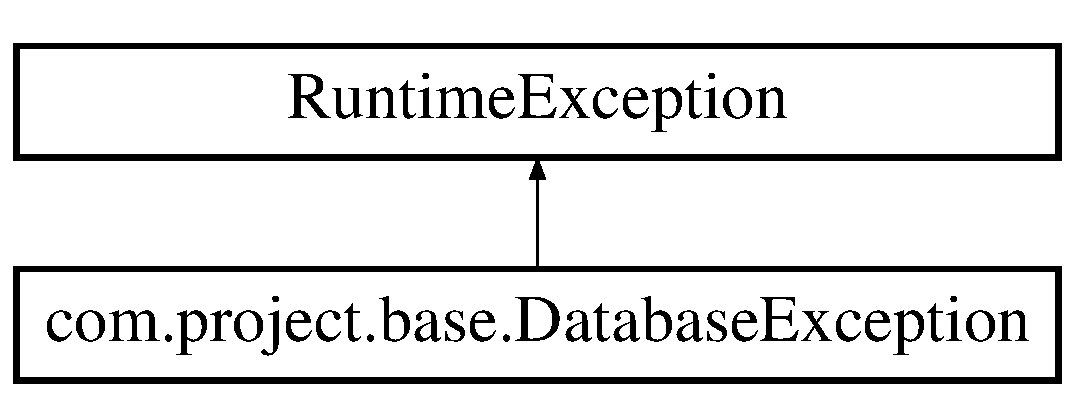
\includegraphics[height=2.000000cm]{classcom_1_1project_1_1base_1_1_database_exception}
\end{center}
\end{figure}
\subsection*{Public Member Functions}
\begin{DoxyCompactItemize}
\item 
\mbox{\label{classcom_1_1project_1_1base_1_1_database_exception_a494e710fd8f0d181db37c3b9ad0f9410}} 
{\bfseries Database\+Exception} (Throwable cause)
\item 
\mbox{\label{classcom_1_1project_1_1base_1_1_database_exception_ac8fc4777486a87669b958b92a836bd14}} 
{\bfseries Database\+Exception} (String message)
\end{DoxyCompactItemize}


\subsection{Detailed Description}
\begin{DoxyAuthor}{Author}
seweryn 
\end{DoxyAuthor}


The documentation for this class was generated from the following file\+:\begin{DoxyCompactItemize}
\item 
/\+Users/seweryn/\+Net\+Beans\+Projects/\+Ceneo\+H\+D/\+Ceneo\+H\+D-\/lib/src/com/project/base/Database\+Exception.\+java\end{DoxyCompactItemize}

\section{com.\+project.\+application.\+Export\+Reviews\+Argument Class Reference}
\label{classcom_1_1project_1_1application_1_1_export_reviews_argument}\index{com.\+project.\+application.\+Export\+Reviews\+Argument@{com.\+project.\+application.\+Export\+Reviews\+Argument}}
\subsection*{Public Member Functions}
\begin{DoxyCompactItemize}
\item 
\textbf{ Export\+Reviews\+Argument} (\textbf{ Export\+Reviews\+Format} format, String file\+Name, String product\+Remote\+Id)
\end{DoxyCompactItemize}
\subsection*{Public Attributes}
\begin{DoxyCompactItemize}
\item 
\mbox{\label{classcom_1_1project_1_1application_1_1_export_reviews_argument_a89f95e67feeb41d396deb4d15b914047}} 
final \textbf{ Export\+Reviews\+Format} {\bfseries format}
\item 
\mbox{\label{classcom_1_1project_1_1application_1_1_export_reviews_argument_af473f24ebdbbe8fd16571ec82b3af6da}} 
final String {\bfseries product\+Remote\+Id}
\item 
\mbox{\label{classcom_1_1project_1_1application_1_1_export_reviews_argument_a4745eb6dadd4c8b0825aa1bb945b0077}} 
final String {\bfseries file\+Name}
\end{DoxyCompactItemize}


\subsection{Detailed Description}
\begin{DoxyAuthor}{Author}
seweryn
\end{DoxyAuthor}
Argument zawierający konfiguracje eksportu opini. 

\subsection{Constructor \& Destructor Documentation}
\mbox{\label{classcom_1_1project_1_1application_1_1_export_reviews_argument_a7e990b328de513bc375b7c2088368fbd}} 
\index{com\+::project\+::application\+::\+Export\+Reviews\+Argument@{com\+::project\+::application\+::\+Export\+Reviews\+Argument}!Export\+Reviews\+Argument@{Export\+Reviews\+Argument}}
\index{Export\+Reviews\+Argument@{Export\+Reviews\+Argument}!com\+::project\+::application\+::\+Export\+Reviews\+Argument@{com\+::project\+::application\+::\+Export\+Reviews\+Argument}}
\subsubsection{Export\+Reviews\+Argument()}
{\footnotesize\ttfamily com.\+project.\+application.\+Export\+Reviews\+Argument.\+Export\+Reviews\+Argument (\begin{DoxyParamCaption}\item[{\textbf{ Export\+Reviews\+Format}}]{format,  }\item[{String}]{file\+Name,  }\item[{String}]{product\+Remote\+Id }\end{DoxyParamCaption})}


\begin{DoxyParams}{Parameters}
{\em format} & -\/ format eksportowanych opini \\
\hline
{\em file\+Name} & -\/ nazwa pliku \\
\hline
{\em product\+Remote\+Id} & -\/ id product to wyeksportowania opini \\
\hline
\end{DoxyParams}


The documentation for this class was generated from the following file\+:\begin{DoxyCompactItemize}
\item 
/\+Users/seweryn/\+Net\+Beans\+Projects/\+Ceneo\+H\+D/\+Ceneo\+H\+D-\/lib/src/com/project/application/Export\+Reviews\+Argument.\+java\end{DoxyCompactItemize}

\section{com.\+project.\+application.\+Export\+Reviews\+Format Enum Reference}
\label{enumcom_1_1project_1_1application_1_1_export_reviews_format}\index{com.\+project.\+application.\+Export\+Reviews\+Format@{com.\+project.\+application.\+Export\+Reviews\+Format}}
\subsection*{Public Attributes}
\begin{DoxyCompactItemize}
\item 
\mbox{\label{enumcom_1_1project_1_1application_1_1_export_reviews_format_a4d2ad6a1843b5cffb661b2baf3017136}} 
{\bfseries T\+XT}
\item 
\mbox{\label{enumcom_1_1project_1_1application_1_1_export_reviews_format_aab38020e1b3526159f16422d5b34afe4}} 
{\bfseries C\+SV}
\end{DoxyCompactItemize}


\subsection{Detailed Description}
\begin{DoxyAuthor}{Author}
seweryn Enum określa format eksportowanych opini. 
\end{DoxyAuthor}


The documentation for this enum was generated from the following file\+:\begin{DoxyCompactItemize}
\item 
/\+Users/seweryn/\+Net\+Beans\+Projects/\+Ceneo\+H\+D/\+Ceneo\+H\+D-\/lib/src/com/project/application/Export\+Reviews\+Format.\+java\end{DoxyCompactItemize}

\section{com.\+project.\+base.\+On\+Error\+Listener Interface Reference}
\label{interfacecom_1_1project_1_1base_1_1_on_error_listener}\index{com.\+project.\+base.\+On\+Error\+Listener@{com.\+project.\+base.\+On\+Error\+Listener}}
\subsection*{Public Member Functions}
\begin{DoxyCompactItemize}
\item 
void \textbf{ on\+Error} (Throwable error)
\end{DoxyCompactItemize}


\subsection{Detailed Description}
\begin{DoxyAuthor}{Author}
seweryn
\end{DoxyAuthor}
Ten interface obsługuje zgłaszanie błędu podczas wykonania \doxyref{Use\+Case}{p.}{interfacecom_1_1project_1_1base_1_1_use_case}\textquotesingle{}a. 

\subsection{Member Function Documentation}
\mbox{\label{interfacecom_1_1project_1_1base_1_1_on_error_listener_a18544d77a758c4a8c9e46bb875c7d773}} 
\index{com\+::project\+::base\+::\+On\+Error\+Listener@{com\+::project\+::base\+::\+On\+Error\+Listener}!on\+Error@{on\+Error}}
\index{on\+Error@{on\+Error}!com\+::project\+::base\+::\+On\+Error\+Listener@{com\+::project\+::base\+::\+On\+Error\+Listener}}
\subsubsection{on\+Error()}
{\footnotesize\ttfamily void com.\+project.\+base.\+On\+Error\+Listener.\+on\+Error (\begin{DoxyParamCaption}\item[{Throwable}]{error }\end{DoxyParamCaption})}


\begin{DoxyParams}{Parameters}
{\em error} & -\/ błąd zgłoszony podczas wykonania operacji \\
\hline
\end{DoxyParams}


The documentation for this interface was generated from the following file\+:\begin{DoxyCompactItemize}
\item 
/\+Users/seweryn/\+Net\+Beans\+Projects/\+Ceneo\+H\+D/\+Ceneo\+H\+D-\/lib/src/com/project/base/On\+Error\+Listener.\+java\end{DoxyCompactItemize}

\section{com.\+project.\+base.\+On\+Success\+Listener$<$ R\+E\+S\+U\+L\+T\+\_\+\+O\+B\+J\+E\+CT $>$ Interface Template Reference}
\label{interfacecom_1_1project_1_1base_1_1_on_success_listener}\index{com.\+project.\+base.\+On\+Success\+Listener$<$ R\+E\+S\+U\+L\+T\+\_\+\+O\+B\+J\+E\+C\+T $>$@{com.\+project.\+base.\+On\+Success\+Listener$<$ R\+E\+S\+U\+L\+T\+\_\+\+O\+B\+J\+E\+C\+T $>$}}
\subsection*{Public Member Functions}
\begin{DoxyCompactItemize}
\item 
void \textbf{ on\+Success} (R\+E\+S\+U\+L\+T\+\_\+\+O\+B\+J\+E\+CT result)
\end{DoxyCompactItemize}


\subsection{Detailed Description}
\begin{DoxyAuthor}{Author}
seweryn
\end{DoxyAuthor}
Ten interface obsługuje wynik operacji wykonania \doxyref{Use\+Case}{p.}{interfacecom_1_1project_1_1base_1_1_use_case}\textquotesingle{}a.


\begin{DoxyParams}{Parameters}
{\em $<$\+R\+E\+S\+U\+L\+T\+\_\+\+O\+B\+J\+E\+C\+T$>$} & -\/ typ wyniku operacji \\
\hline
\end{DoxyParams}


\subsection{Member Function Documentation}
\mbox{\label{interfacecom_1_1project_1_1base_1_1_on_success_listener_a0d434e0bc4bf04925e8c276157e877f3}} 
\index{com\+::project\+::base\+::\+On\+Success\+Listener@{com\+::project\+::base\+::\+On\+Success\+Listener}!on\+Success@{on\+Success}}
\index{on\+Success@{on\+Success}!com\+::project\+::base\+::\+On\+Success\+Listener@{com\+::project\+::base\+::\+On\+Success\+Listener}}
\subsubsection{on\+Success()}
{\footnotesize\ttfamily void \textbf{ com.\+project.\+base.\+On\+Success\+Listener}$<$ R\+E\+S\+U\+L\+T\+\_\+\+O\+B\+J\+E\+CT $>$.on\+Success (\begin{DoxyParamCaption}\item[{R\+E\+S\+U\+L\+T\+\_\+\+O\+B\+J\+E\+CT}]{result }\end{DoxyParamCaption})}


\begin{DoxyParams}{Parameters}
{\em result} & wynik operacji \\
\hline
\end{DoxyParams}


The documentation for this interface was generated from the following file\+:\begin{DoxyCompactItemize}
\item 
/\+Users/seweryn/\+Net\+Beans\+Projects/\+Ceneo\+H\+D/\+Ceneo\+H\+D-\/lib/src/com/project/base/On\+Success\+Listener.\+java\end{DoxyCompactItemize}

\section{com.\+project.\+dto.\+Product\+D\+TO Class Reference}
\label{classcom_1_1project_1_1dto_1_1_product_d_t_o}\index{com.\+project.\+dto.\+Product\+D\+TO@{com.\+project.\+dto.\+Product\+D\+TO}}
\subsection*{Public Member Functions}
\begin{DoxyCompactItemize}
\item 
\textbf{ Product\+D\+TO} ()
\item 
\textbf{ Product\+D\+TO} (String remote\+Id)
\item 
String \textbf{ get\+Remote\+Id} ()
\item 
void \textbf{ set\+Remote\+Id} (String remote\+Id)
\item 
String \textbf{ get\+Category} ()
\item 
void \textbf{ set\+Category} (String category)
\item 
String \textbf{ get\+Name} ()
\item 
void \textbf{ set\+Name} (String name)
\item 
String \textbf{ get\+Params} ()
\item 
void \textbf{ set\+Params} (String params)
\item 
String \textbf{ get\+Price} ()
\item 
void \textbf{ set\+Price} (String price)
\item 
Double \textbf{ get\+Score} ()
\item 
void \textbf{ set\+Score} (Double score)
\item 
String \textbf{ get\+Reviews\+Desc} ()
\item 
void \textbf{ set\+Reviews\+Desc} (String reviews\+Desc)
\end{DoxyCompactItemize}


\subsection{Detailed Description}
\begin{DoxyAuthor}{Author}
seweryn
\end{DoxyAuthor}
Struktura D\+TO przechowująca dane produktu. 

\subsection{Constructor \& Destructor Documentation}
\mbox{\label{classcom_1_1project_1_1dto_1_1_product_d_t_o_a8d5348e0560b604f30128393b56f2c80}} 
\index{com\+::project\+::dto\+::\+Product\+D\+TO@{com\+::project\+::dto\+::\+Product\+D\+TO}!Product\+D\+TO@{Product\+D\+TO}}
\index{Product\+D\+TO@{Product\+D\+TO}!com\+::project\+::dto\+::\+Product\+D\+TO@{com\+::project\+::dto\+::\+Product\+D\+TO}}
\subsubsection{Product\+D\+T\+O()\hspace{0.1cm}{\footnotesize\ttfamily [1/2]}}
{\footnotesize\ttfamily com.\+project.\+dto.\+Product\+D\+T\+O.\+Product\+D\+TO (\begin{DoxyParamCaption}{ }\end{DoxyParamCaption})}

Konstruktor domyślny \mbox{\label{classcom_1_1project_1_1dto_1_1_product_d_t_o_ad5da33e2cdc64792ca4f6285c51c2ccc}} 
\index{com\+::project\+::dto\+::\+Product\+D\+TO@{com\+::project\+::dto\+::\+Product\+D\+TO}!Product\+D\+TO@{Product\+D\+TO}}
\index{Product\+D\+TO@{Product\+D\+TO}!com\+::project\+::dto\+::\+Product\+D\+TO@{com\+::project\+::dto\+::\+Product\+D\+TO}}
\subsubsection{Product\+D\+T\+O()\hspace{0.1cm}{\footnotesize\ttfamily [2/2]}}
{\footnotesize\ttfamily com.\+project.\+dto.\+Product\+D\+T\+O.\+Product\+D\+TO (\begin{DoxyParamCaption}\item[{String}]{remote\+Id }\end{DoxyParamCaption})}


\begin{DoxyParams}{Parameters}
{\em remote\+Id} & zdalne id produktu \\
\hline
\end{DoxyParams}


\subsection{Member Function Documentation}
\mbox{\label{classcom_1_1project_1_1dto_1_1_product_d_t_o_a23adcdd63df3545bb305456a880d39e3}} 
\index{com\+::project\+::dto\+::\+Product\+D\+TO@{com\+::project\+::dto\+::\+Product\+D\+TO}!get\+Category@{get\+Category}}
\index{get\+Category@{get\+Category}!com\+::project\+::dto\+::\+Product\+D\+TO@{com\+::project\+::dto\+::\+Product\+D\+TO}}
\subsubsection{get\+Category()}
{\footnotesize\ttfamily String com.\+project.\+dto.\+Product\+D\+T\+O.\+get\+Category (\begin{DoxyParamCaption}{ }\end{DoxyParamCaption})}

\begin{DoxyReturn}{Returns}
kategoria 
\end{DoxyReturn}
\mbox{\label{classcom_1_1project_1_1dto_1_1_product_d_t_o_a0c491526298f74ee43962ec79dc233fd}} 
\index{com\+::project\+::dto\+::\+Product\+D\+TO@{com\+::project\+::dto\+::\+Product\+D\+TO}!get\+Name@{get\+Name}}
\index{get\+Name@{get\+Name}!com\+::project\+::dto\+::\+Product\+D\+TO@{com\+::project\+::dto\+::\+Product\+D\+TO}}
\subsubsection{get\+Name()}
{\footnotesize\ttfamily String com.\+project.\+dto.\+Product\+D\+T\+O.\+get\+Name (\begin{DoxyParamCaption}{ }\end{DoxyParamCaption})}

\begin{DoxyReturn}{Returns}
nazwa 
\end{DoxyReturn}
\mbox{\label{classcom_1_1project_1_1dto_1_1_product_d_t_o_af3625c281faaa57de016bf742221cdae}} 
\index{com\+::project\+::dto\+::\+Product\+D\+TO@{com\+::project\+::dto\+::\+Product\+D\+TO}!get\+Params@{get\+Params}}
\index{get\+Params@{get\+Params}!com\+::project\+::dto\+::\+Product\+D\+TO@{com\+::project\+::dto\+::\+Product\+D\+TO}}
\subsubsection{get\+Params()}
{\footnotesize\ttfamily String com.\+project.\+dto.\+Product\+D\+T\+O.\+get\+Params (\begin{DoxyParamCaption}{ }\end{DoxyParamCaption})}

\begin{DoxyReturn}{Returns}
parametry 
\end{DoxyReturn}
\mbox{\label{classcom_1_1project_1_1dto_1_1_product_d_t_o_aef28d9f2898e0546b0b115aed3e19046}} 
\index{com\+::project\+::dto\+::\+Product\+D\+TO@{com\+::project\+::dto\+::\+Product\+D\+TO}!get\+Price@{get\+Price}}
\index{get\+Price@{get\+Price}!com\+::project\+::dto\+::\+Product\+D\+TO@{com\+::project\+::dto\+::\+Product\+D\+TO}}
\subsubsection{get\+Price()}
{\footnotesize\ttfamily String com.\+project.\+dto.\+Product\+D\+T\+O.\+get\+Price (\begin{DoxyParamCaption}{ }\end{DoxyParamCaption})}

\begin{DoxyReturn}{Returns}
cena 
\end{DoxyReturn}
\mbox{\label{classcom_1_1project_1_1dto_1_1_product_d_t_o_a378c6cbbca6e335bf6220dfb9554696b}} 
\index{com\+::project\+::dto\+::\+Product\+D\+TO@{com\+::project\+::dto\+::\+Product\+D\+TO}!get\+Remote\+Id@{get\+Remote\+Id}}
\index{get\+Remote\+Id@{get\+Remote\+Id}!com\+::project\+::dto\+::\+Product\+D\+TO@{com\+::project\+::dto\+::\+Product\+D\+TO}}
\subsubsection{get\+Remote\+Id()}
{\footnotesize\ttfamily String com.\+project.\+dto.\+Product\+D\+T\+O.\+get\+Remote\+Id (\begin{DoxyParamCaption}{ }\end{DoxyParamCaption})}

\begin{DoxyReturn}{Returns}
zdalne id produktu 
\end{DoxyReturn}
\mbox{\label{classcom_1_1project_1_1dto_1_1_product_d_t_o_a933d655934ceb8340c7e1671a57f2774}} 
\index{com\+::project\+::dto\+::\+Product\+D\+TO@{com\+::project\+::dto\+::\+Product\+D\+TO}!get\+Reviews\+Desc@{get\+Reviews\+Desc}}
\index{get\+Reviews\+Desc@{get\+Reviews\+Desc}!com\+::project\+::dto\+::\+Product\+D\+TO@{com\+::project\+::dto\+::\+Product\+D\+TO}}
\subsubsection{get\+Reviews\+Desc()}
{\footnotesize\ttfamily String com.\+project.\+dto.\+Product\+D\+T\+O.\+get\+Reviews\+Desc (\begin{DoxyParamCaption}{ }\end{DoxyParamCaption})}

\begin{DoxyReturn}{Returns}
opis opini 
\end{DoxyReturn}
\mbox{\label{classcom_1_1project_1_1dto_1_1_product_d_t_o_acab206bddf31bc2ac61593658df21a80}} 
\index{com\+::project\+::dto\+::\+Product\+D\+TO@{com\+::project\+::dto\+::\+Product\+D\+TO}!get\+Score@{get\+Score}}
\index{get\+Score@{get\+Score}!com\+::project\+::dto\+::\+Product\+D\+TO@{com\+::project\+::dto\+::\+Product\+D\+TO}}
\subsubsection{get\+Score()}
{\footnotesize\ttfamily Double com.\+project.\+dto.\+Product\+D\+T\+O.\+get\+Score (\begin{DoxyParamCaption}{ }\end{DoxyParamCaption})}

\begin{DoxyReturn}{Returns}
średnia ocena 
\end{DoxyReturn}
\mbox{\label{classcom_1_1project_1_1dto_1_1_product_d_t_o_a7c7eec99e2bf4bb4dd209ac9ac9bd8bd}} 
\index{com\+::project\+::dto\+::\+Product\+D\+TO@{com\+::project\+::dto\+::\+Product\+D\+TO}!set\+Category@{set\+Category}}
\index{set\+Category@{set\+Category}!com\+::project\+::dto\+::\+Product\+D\+TO@{com\+::project\+::dto\+::\+Product\+D\+TO}}
\subsubsection{set\+Category()}
{\footnotesize\ttfamily void com.\+project.\+dto.\+Product\+D\+T\+O.\+set\+Category (\begin{DoxyParamCaption}\item[{String}]{category }\end{DoxyParamCaption})}


\begin{DoxyParams}{Parameters}
{\em category} & kategoria \\
\hline
\end{DoxyParams}
\mbox{\label{classcom_1_1project_1_1dto_1_1_product_d_t_o_a56758c0bba18386d8581b7108997f7ac}} 
\index{com\+::project\+::dto\+::\+Product\+D\+TO@{com\+::project\+::dto\+::\+Product\+D\+TO}!set\+Name@{set\+Name}}
\index{set\+Name@{set\+Name}!com\+::project\+::dto\+::\+Product\+D\+TO@{com\+::project\+::dto\+::\+Product\+D\+TO}}
\subsubsection{set\+Name()}
{\footnotesize\ttfamily void com.\+project.\+dto.\+Product\+D\+T\+O.\+set\+Name (\begin{DoxyParamCaption}\item[{String}]{name }\end{DoxyParamCaption})}


\begin{DoxyParams}{Parameters}
{\em name} & nazwa \\
\hline
\end{DoxyParams}
\mbox{\label{classcom_1_1project_1_1dto_1_1_product_d_t_o_a3d1861ed5dfed6287219c2e258f3698b}} 
\index{com\+::project\+::dto\+::\+Product\+D\+TO@{com\+::project\+::dto\+::\+Product\+D\+TO}!set\+Params@{set\+Params}}
\index{set\+Params@{set\+Params}!com\+::project\+::dto\+::\+Product\+D\+TO@{com\+::project\+::dto\+::\+Product\+D\+TO}}
\subsubsection{set\+Params()}
{\footnotesize\ttfamily void com.\+project.\+dto.\+Product\+D\+T\+O.\+set\+Params (\begin{DoxyParamCaption}\item[{String}]{params }\end{DoxyParamCaption})}


\begin{DoxyParams}{Parameters}
{\em params} & parametry \\
\hline
\end{DoxyParams}
\mbox{\label{classcom_1_1project_1_1dto_1_1_product_d_t_o_a686b9454496378446bb8f0b8a3254122}} 
\index{com\+::project\+::dto\+::\+Product\+D\+TO@{com\+::project\+::dto\+::\+Product\+D\+TO}!set\+Price@{set\+Price}}
\index{set\+Price@{set\+Price}!com\+::project\+::dto\+::\+Product\+D\+TO@{com\+::project\+::dto\+::\+Product\+D\+TO}}
\subsubsection{set\+Price()}
{\footnotesize\ttfamily void com.\+project.\+dto.\+Product\+D\+T\+O.\+set\+Price (\begin{DoxyParamCaption}\item[{String}]{price }\end{DoxyParamCaption})}


\begin{DoxyParams}{Parameters}
{\em price} & cena \\
\hline
\end{DoxyParams}
\mbox{\label{classcom_1_1project_1_1dto_1_1_product_d_t_o_a67d3344a5f5c709217c74db630e22eab}} 
\index{com\+::project\+::dto\+::\+Product\+D\+TO@{com\+::project\+::dto\+::\+Product\+D\+TO}!set\+Remote\+Id@{set\+Remote\+Id}}
\index{set\+Remote\+Id@{set\+Remote\+Id}!com\+::project\+::dto\+::\+Product\+D\+TO@{com\+::project\+::dto\+::\+Product\+D\+TO}}
\subsubsection{set\+Remote\+Id()}
{\footnotesize\ttfamily void com.\+project.\+dto.\+Product\+D\+T\+O.\+set\+Remote\+Id (\begin{DoxyParamCaption}\item[{String}]{remote\+Id }\end{DoxyParamCaption})}


\begin{DoxyParams}{Parameters}
{\em remote\+Id} & zdalne id produktu \\
\hline
\end{DoxyParams}
\mbox{\label{classcom_1_1project_1_1dto_1_1_product_d_t_o_a629eff74a4ebb22acd06e5241ae61c61}} 
\index{com\+::project\+::dto\+::\+Product\+D\+TO@{com\+::project\+::dto\+::\+Product\+D\+TO}!set\+Reviews\+Desc@{set\+Reviews\+Desc}}
\index{set\+Reviews\+Desc@{set\+Reviews\+Desc}!com\+::project\+::dto\+::\+Product\+D\+TO@{com\+::project\+::dto\+::\+Product\+D\+TO}}
\subsubsection{set\+Reviews\+Desc()}
{\footnotesize\ttfamily void com.\+project.\+dto.\+Product\+D\+T\+O.\+set\+Reviews\+Desc (\begin{DoxyParamCaption}\item[{String}]{reviews\+Desc }\end{DoxyParamCaption})}


\begin{DoxyParams}{Parameters}
{\em reviews\+Desc} & opis opini \\
\hline
\end{DoxyParams}
\mbox{\label{classcom_1_1project_1_1dto_1_1_product_d_t_o_a17541864e8cfff6303e958139eb1a3a9}} 
\index{com\+::project\+::dto\+::\+Product\+D\+TO@{com\+::project\+::dto\+::\+Product\+D\+TO}!set\+Score@{set\+Score}}
\index{set\+Score@{set\+Score}!com\+::project\+::dto\+::\+Product\+D\+TO@{com\+::project\+::dto\+::\+Product\+D\+TO}}
\subsubsection{set\+Score()}
{\footnotesize\ttfamily void com.\+project.\+dto.\+Product\+D\+T\+O.\+set\+Score (\begin{DoxyParamCaption}\item[{Double}]{score }\end{DoxyParamCaption})}


\begin{DoxyParams}{Parameters}
{\em score} & średnia ocena \\
\hline
\end{DoxyParams}


The documentation for this class was generated from the following file\+:\begin{DoxyCompactItemize}
\item 
/\+Users/seweryn/\+Net\+Beans\+Projects/\+Ceneo\+H\+D/\+Ceneo\+H\+D-\/lib/src/com/project/dto/Product\+D\+T\+O.\+java\end{DoxyCompactItemize}

\section{com.\+project.\+entity.\+Product\+Entity Class Reference}
\label{classcom_1_1project_1_1entity_1_1_product_entity}\index{com.\+project.\+entity.\+Product\+Entity@{com.\+project.\+entity.\+Product\+Entity}}
\subsection*{Public Member Functions}
\begin{DoxyCompactItemize}
\item 
\textbf{ Product\+Entity} ()
\item 
\textbf{ Product\+Entity} (String remote\+Id, String category, String name, String params, String price, Double score, String reviews\+Desc)
\item 
Long \textbf{ get\+Id} ()
\item 
String \textbf{ get\+Remote\+Id} ()
\item 
void \textbf{ set\+Reviews} (Collection$<$ \textbf{ Review\+Entity} $>$ reviews)
\item 
Collection$<$ \textbf{ Review\+Entity} $>$ \textbf{ get\+Reviews} ()
\item 
void \textbf{ set\+Id} (Long id)
\item 
String \textbf{ get\+Category} ()
\item 
void \textbf{ set\+Category} (String category)
\item 
String \textbf{ get\+Name} ()
\item 
void \textbf{ set\+Name} (String name)
\item 
String \textbf{ get\+Params} ()
\item 
void \textbf{ set\+Params} (String params)
\item 
String \textbf{ get\+Price} ()
\item 
void \textbf{ set\+Price} (String price)
\item 
Double \textbf{ get\+Score} ()
\item 
void \textbf{ set\+Score} (Double score)
\item 
String \textbf{ get\+Reviews\+Desc} ()
\item 
void \textbf{ set\+Reviews\+Desc} (String reviews\+Desc)
\end{DoxyCompactItemize}


\subsection{Detailed Description}
\begin{DoxyAuthor}{Author}
seweryn
\end{DoxyAuthor}
Encja definiująca tabelę produktów w bazie danych. 

\subsection{Constructor \& Destructor Documentation}
\mbox{\label{classcom_1_1project_1_1entity_1_1_product_entity_a0de3d4840ff34f9086537cfc2f3bf64d}} 
\index{com\+::project\+::entity\+::\+Product\+Entity@{com\+::project\+::entity\+::\+Product\+Entity}!Product\+Entity@{Product\+Entity}}
\index{Product\+Entity@{Product\+Entity}!com\+::project\+::entity\+::\+Product\+Entity@{com\+::project\+::entity\+::\+Product\+Entity}}
\subsubsection{Product\+Entity()\hspace{0.1cm}{\footnotesize\ttfamily [1/2]}}
{\footnotesize\ttfamily com.\+project.\+entity.\+Product\+Entity.\+Product\+Entity (\begin{DoxyParamCaption}{ }\end{DoxyParamCaption})}

Konstruktor domyślny \mbox{\label{classcom_1_1project_1_1entity_1_1_product_entity_aba38dd9899f49476f1c13900ba95ff25}} 
\index{com\+::project\+::entity\+::\+Product\+Entity@{com\+::project\+::entity\+::\+Product\+Entity}!Product\+Entity@{Product\+Entity}}
\index{Product\+Entity@{Product\+Entity}!com\+::project\+::entity\+::\+Product\+Entity@{com\+::project\+::entity\+::\+Product\+Entity}}
\subsubsection{Product\+Entity()\hspace{0.1cm}{\footnotesize\ttfamily [2/2]}}
{\footnotesize\ttfamily com.\+project.\+entity.\+Product\+Entity.\+Product\+Entity (\begin{DoxyParamCaption}\item[{String}]{remote\+Id,  }\item[{String}]{category,  }\item[{String}]{name,  }\item[{String}]{params,  }\item[{String}]{price,  }\item[{Double}]{score,  }\item[{String}]{reviews\+Desc }\end{DoxyParamCaption})}


\begin{DoxyParams}{Parameters}
{\em remote\+Id} & \\
\hline
{\em category} & \\
\hline
{\em name} & \\
\hline
{\em params} & \\
\hline
{\em price} & \\
\hline
{\em score} & \\
\hline
{\em reviews\+Desc} & \\
\hline
\end{DoxyParams}


\subsection{Member Function Documentation}
\mbox{\label{classcom_1_1project_1_1entity_1_1_product_entity_a001fa9344b152d474aacea83aad4d5c9}} 
\index{com\+::project\+::entity\+::\+Product\+Entity@{com\+::project\+::entity\+::\+Product\+Entity}!get\+Category@{get\+Category}}
\index{get\+Category@{get\+Category}!com\+::project\+::entity\+::\+Product\+Entity@{com\+::project\+::entity\+::\+Product\+Entity}}
\subsubsection{get\+Category()}
{\footnotesize\ttfamily String com.\+project.\+entity.\+Product\+Entity.\+get\+Category (\begin{DoxyParamCaption}{ }\end{DoxyParamCaption})}

\begin{DoxyReturn}{Returns}

\end{DoxyReturn}
\mbox{\label{classcom_1_1project_1_1entity_1_1_product_entity_a93a5bdbed17d2c26ce0ceeaf3a4c12cc}} 
\index{com\+::project\+::entity\+::\+Product\+Entity@{com\+::project\+::entity\+::\+Product\+Entity}!get\+Id@{get\+Id}}
\index{get\+Id@{get\+Id}!com\+::project\+::entity\+::\+Product\+Entity@{com\+::project\+::entity\+::\+Product\+Entity}}
\subsubsection{get\+Id()}
{\footnotesize\ttfamily Long com.\+project.\+entity.\+Product\+Entity.\+get\+Id (\begin{DoxyParamCaption}{ }\end{DoxyParamCaption})}

\begin{DoxyReturn}{Returns}

\end{DoxyReturn}
\mbox{\label{classcom_1_1project_1_1entity_1_1_product_entity_a4e67cb7a866bfc4b2079fbf4699ff677}} 
\index{com\+::project\+::entity\+::\+Product\+Entity@{com\+::project\+::entity\+::\+Product\+Entity}!get\+Name@{get\+Name}}
\index{get\+Name@{get\+Name}!com\+::project\+::entity\+::\+Product\+Entity@{com\+::project\+::entity\+::\+Product\+Entity}}
\subsubsection{get\+Name()}
{\footnotesize\ttfamily String com.\+project.\+entity.\+Product\+Entity.\+get\+Name (\begin{DoxyParamCaption}{ }\end{DoxyParamCaption})}

\begin{DoxyReturn}{Returns}

\end{DoxyReturn}
\mbox{\label{classcom_1_1project_1_1entity_1_1_product_entity_aef6b7bb6964cdf7faba21432ce7186be}} 
\index{com\+::project\+::entity\+::\+Product\+Entity@{com\+::project\+::entity\+::\+Product\+Entity}!get\+Params@{get\+Params}}
\index{get\+Params@{get\+Params}!com\+::project\+::entity\+::\+Product\+Entity@{com\+::project\+::entity\+::\+Product\+Entity}}
\subsubsection{get\+Params()}
{\footnotesize\ttfamily String com.\+project.\+entity.\+Product\+Entity.\+get\+Params (\begin{DoxyParamCaption}{ }\end{DoxyParamCaption})}

\begin{DoxyReturn}{Returns}

\end{DoxyReturn}
\mbox{\label{classcom_1_1project_1_1entity_1_1_product_entity_a963b495812a31075069f851dcb004367}} 
\index{com\+::project\+::entity\+::\+Product\+Entity@{com\+::project\+::entity\+::\+Product\+Entity}!get\+Price@{get\+Price}}
\index{get\+Price@{get\+Price}!com\+::project\+::entity\+::\+Product\+Entity@{com\+::project\+::entity\+::\+Product\+Entity}}
\subsubsection{get\+Price()}
{\footnotesize\ttfamily String com.\+project.\+entity.\+Product\+Entity.\+get\+Price (\begin{DoxyParamCaption}{ }\end{DoxyParamCaption})}

\begin{DoxyReturn}{Returns}

\end{DoxyReturn}
\mbox{\label{classcom_1_1project_1_1entity_1_1_product_entity_ae1c32fcfee92a656ec45f983eb335be1}} 
\index{com\+::project\+::entity\+::\+Product\+Entity@{com\+::project\+::entity\+::\+Product\+Entity}!get\+Remote\+Id@{get\+Remote\+Id}}
\index{get\+Remote\+Id@{get\+Remote\+Id}!com\+::project\+::entity\+::\+Product\+Entity@{com\+::project\+::entity\+::\+Product\+Entity}}
\subsubsection{get\+Remote\+Id()}
{\footnotesize\ttfamily String com.\+project.\+entity.\+Product\+Entity.\+get\+Remote\+Id (\begin{DoxyParamCaption}{ }\end{DoxyParamCaption})}

\begin{DoxyReturn}{Returns}

\end{DoxyReturn}
\mbox{\label{classcom_1_1project_1_1entity_1_1_product_entity_ae95f09c819ffe006739c370b85e9d2c1}} 
\index{com\+::project\+::entity\+::\+Product\+Entity@{com\+::project\+::entity\+::\+Product\+Entity}!get\+Reviews@{get\+Reviews}}
\index{get\+Reviews@{get\+Reviews}!com\+::project\+::entity\+::\+Product\+Entity@{com\+::project\+::entity\+::\+Product\+Entity}}
\subsubsection{get\+Reviews()}
{\footnotesize\ttfamily Collection$<$\textbf{ Review\+Entity}$>$ com.\+project.\+entity.\+Product\+Entity.\+get\+Reviews (\begin{DoxyParamCaption}{ }\end{DoxyParamCaption})}

\begin{DoxyReturn}{Returns}

\end{DoxyReturn}
\mbox{\label{classcom_1_1project_1_1entity_1_1_product_entity_abaa80a3a3ba07232f7582bb3425bd3fb}} 
\index{com\+::project\+::entity\+::\+Product\+Entity@{com\+::project\+::entity\+::\+Product\+Entity}!get\+Reviews\+Desc@{get\+Reviews\+Desc}}
\index{get\+Reviews\+Desc@{get\+Reviews\+Desc}!com\+::project\+::entity\+::\+Product\+Entity@{com\+::project\+::entity\+::\+Product\+Entity}}
\subsubsection{get\+Reviews\+Desc()}
{\footnotesize\ttfamily String com.\+project.\+entity.\+Product\+Entity.\+get\+Reviews\+Desc (\begin{DoxyParamCaption}{ }\end{DoxyParamCaption})}

\begin{DoxyReturn}{Returns}

\end{DoxyReturn}
\mbox{\label{classcom_1_1project_1_1entity_1_1_product_entity_a3a160d22e0809d2a749cb72fe5af10d6}} 
\index{com\+::project\+::entity\+::\+Product\+Entity@{com\+::project\+::entity\+::\+Product\+Entity}!get\+Score@{get\+Score}}
\index{get\+Score@{get\+Score}!com\+::project\+::entity\+::\+Product\+Entity@{com\+::project\+::entity\+::\+Product\+Entity}}
\subsubsection{get\+Score()}
{\footnotesize\ttfamily Double com.\+project.\+entity.\+Product\+Entity.\+get\+Score (\begin{DoxyParamCaption}{ }\end{DoxyParamCaption})}

\begin{DoxyReturn}{Returns}

\end{DoxyReturn}
\mbox{\label{classcom_1_1project_1_1entity_1_1_product_entity_ac8381c47957fa468dc419f670a4fe40b}} 
\index{com\+::project\+::entity\+::\+Product\+Entity@{com\+::project\+::entity\+::\+Product\+Entity}!set\+Category@{set\+Category}}
\index{set\+Category@{set\+Category}!com\+::project\+::entity\+::\+Product\+Entity@{com\+::project\+::entity\+::\+Product\+Entity}}
\subsubsection{set\+Category()}
{\footnotesize\ttfamily void com.\+project.\+entity.\+Product\+Entity.\+set\+Category (\begin{DoxyParamCaption}\item[{String}]{category }\end{DoxyParamCaption})}


\begin{DoxyParams}{Parameters}
{\em category} & \\
\hline
\end{DoxyParams}
\mbox{\label{classcom_1_1project_1_1entity_1_1_product_entity_a903bf91b6799ea6d78ca1db647342ec5}} 
\index{com\+::project\+::entity\+::\+Product\+Entity@{com\+::project\+::entity\+::\+Product\+Entity}!set\+Id@{set\+Id}}
\index{set\+Id@{set\+Id}!com\+::project\+::entity\+::\+Product\+Entity@{com\+::project\+::entity\+::\+Product\+Entity}}
\subsubsection{set\+Id()}
{\footnotesize\ttfamily void com.\+project.\+entity.\+Product\+Entity.\+set\+Id (\begin{DoxyParamCaption}\item[{Long}]{id }\end{DoxyParamCaption})}


\begin{DoxyParams}{Parameters}
{\em id} & \\
\hline
\end{DoxyParams}
\mbox{\label{classcom_1_1project_1_1entity_1_1_product_entity_acea1f2baa2e7e2517c0d8705396b4bd4}} 
\index{com\+::project\+::entity\+::\+Product\+Entity@{com\+::project\+::entity\+::\+Product\+Entity}!set\+Name@{set\+Name}}
\index{set\+Name@{set\+Name}!com\+::project\+::entity\+::\+Product\+Entity@{com\+::project\+::entity\+::\+Product\+Entity}}
\subsubsection{set\+Name()}
{\footnotesize\ttfamily void com.\+project.\+entity.\+Product\+Entity.\+set\+Name (\begin{DoxyParamCaption}\item[{String}]{name }\end{DoxyParamCaption})}


\begin{DoxyParams}{Parameters}
{\em name} & \\
\hline
\end{DoxyParams}
\mbox{\label{classcom_1_1project_1_1entity_1_1_product_entity_a0c4bd4b2b74e864259780f401540da11}} 
\index{com\+::project\+::entity\+::\+Product\+Entity@{com\+::project\+::entity\+::\+Product\+Entity}!set\+Params@{set\+Params}}
\index{set\+Params@{set\+Params}!com\+::project\+::entity\+::\+Product\+Entity@{com\+::project\+::entity\+::\+Product\+Entity}}
\subsubsection{set\+Params()}
{\footnotesize\ttfamily void com.\+project.\+entity.\+Product\+Entity.\+set\+Params (\begin{DoxyParamCaption}\item[{String}]{params }\end{DoxyParamCaption})}


\begin{DoxyParams}{Parameters}
{\em params} & \\
\hline
\end{DoxyParams}
\mbox{\label{classcom_1_1project_1_1entity_1_1_product_entity_a5160f5c66011013b9f5a9eee2a953da7}} 
\index{com\+::project\+::entity\+::\+Product\+Entity@{com\+::project\+::entity\+::\+Product\+Entity}!set\+Price@{set\+Price}}
\index{set\+Price@{set\+Price}!com\+::project\+::entity\+::\+Product\+Entity@{com\+::project\+::entity\+::\+Product\+Entity}}
\subsubsection{set\+Price()}
{\footnotesize\ttfamily void com.\+project.\+entity.\+Product\+Entity.\+set\+Price (\begin{DoxyParamCaption}\item[{String}]{price }\end{DoxyParamCaption})}


\begin{DoxyParams}{Parameters}
{\em price} & \\
\hline
\end{DoxyParams}
\mbox{\label{classcom_1_1project_1_1entity_1_1_product_entity_ab159b3e6514806ddd7b06ea04fff8614}} 
\index{com\+::project\+::entity\+::\+Product\+Entity@{com\+::project\+::entity\+::\+Product\+Entity}!set\+Reviews@{set\+Reviews}}
\index{set\+Reviews@{set\+Reviews}!com\+::project\+::entity\+::\+Product\+Entity@{com\+::project\+::entity\+::\+Product\+Entity}}
\subsubsection{set\+Reviews()}
{\footnotesize\ttfamily void com.\+project.\+entity.\+Product\+Entity.\+set\+Reviews (\begin{DoxyParamCaption}\item[{Collection$<$ \textbf{ Review\+Entity} $>$}]{reviews }\end{DoxyParamCaption})}


\begin{DoxyParams}{Parameters}
{\em reviews} & \\
\hline
\end{DoxyParams}
\mbox{\label{classcom_1_1project_1_1entity_1_1_product_entity_ad39b3fb1e39e5006a4d750f574782679}} 
\index{com\+::project\+::entity\+::\+Product\+Entity@{com\+::project\+::entity\+::\+Product\+Entity}!set\+Reviews\+Desc@{set\+Reviews\+Desc}}
\index{set\+Reviews\+Desc@{set\+Reviews\+Desc}!com\+::project\+::entity\+::\+Product\+Entity@{com\+::project\+::entity\+::\+Product\+Entity}}
\subsubsection{set\+Reviews\+Desc()}
{\footnotesize\ttfamily void com.\+project.\+entity.\+Product\+Entity.\+set\+Reviews\+Desc (\begin{DoxyParamCaption}\item[{String}]{reviews\+Desc }\end{DoxyParamCaption})}


\begin{DoxyParams}{Parameters}
{\em reviews\+Desc} & \\
\hline
\end{DoxyParams}
\mbox{\label{classcom_1_1project_1_1entity_1_1_product_entity_a24bfeeaceb2692373ceb96351fea0bba}} 
\index{com\+::project\+::entity\+::\+Product\+Entity@{com\+::project\+::entity\+::\+Product\+Entity}!set\+Score@{set\+Score}}
\index{set\+Score@{set\+Score}!com\+::project\+::entity\+::\+Product\+Entity@{com\+::project\+::entity\+::\+Product\+Entity}}
\subsubsection{set\+Score()}
{\footnotesize\ttfamily void com.\+project.\+entity.\+Product\+Entity.\+set\+Score (\begin{DoxyParamCaption}\item[{Double}]{score }\end{DoxyParamCaption})}


\begin{DoxyParams}{Parameters}
{\em score} & \\
\hline
\end{DoxyParams}


The documentation for this class was generated from the following file\+:\begin{DoxyCompactItemize}
\item 
/\+Users/seweryn/\+Net\+Beans\+Projects/\+Ceneo\+H\+D/\+Ceneo\+H\+D-\/lib/src/com/project/entity/Product\+Entity.\+java\end{DoxyCompactItemize}

\section{com.\+project.\+dto.\+Product\+Reviews\+D\+TO Class Reference}
\label{classcom_1_1project_1_1dto_1_1_product_reviews_d_t_o}\index{com.\+project.\+dto.\+Product\+Reviews\+D\+TO@{com.\+project.\+dto.\+Product\+Reviews\+D\+TO}}
\subsection*{Public Member Functions}
\begin{DoxyCompactItemize}
\item 
\textbf{ Product\+Reviews\+D\+TO} (\textbf{ Product\+D\+TO} product, Collection$<$ \textbf{ Review\+D\+TO} $>$ reviews)
\item 
\textbf{ Product\+D\+TO} \textbf{ get\+Product} ()
\item 
Collection$<$ \textbf{ Review\+D\+TO} $>$ \textbf{ get\+Reviews} ()
\end{DoxyCompactItemize}


\subsection{Detailed Description}
\begin{DoxyAuthor}{Author}
seweryn
\end{DoxyAuthor}
Struktura D\+TO przechowująca obiekt z danymi produktu oraz jego listą opini. 

\subsection{Constructor \& Destructor Documentation}
\mbox{\label{classcom_1_1project_1_1dto_1_1_product_reviews_d_t_o_ac97203e6e115fa53605429652ddda9da}} 
\index{com\+::project\+::dto\+::\+Product\+Reviews\+D\+TO@{com\+::project\+::dto\+::\+Product\+Reviews\+D\+TO}!Product\+Reviews\+D\+TO@{Product\+Reviews\+D\+TO}}
\index{Product\+Reviews\+D\+TO@{Product\+Reviews\+D\+TO}!com\+::project\+::dto\+::\+Product\+Reviews\+D\+TO@{com\+::project\+::dto\+::\+Product\+Reviews\+D\+TO}}
\subsubsection{Product\+Reviews\+D\+T\+O()}
{\footnotesize\ttfamily com.\+project.\+dto.\+Product\+Reviews\+D\+T\+O.\+Product\+Reviews\+D\+TO (\begin{DoxyParamCaption}\item[{\textbf{ Product\+D\+TO}}]{product,  }\item[{Collection$<$ \textbf{ Review\+D\+TO} $>$}]{reviews }\end{DoxyParamCaption})}


\begin{DoxyParams}{Parameters}
{\em product} & dane produktu \\
\hline
{\em reviews} & lista opini \\
\hline
\end{DoxyParams}


\subsection{Member Function Documentation}
\mbox{\label{classcom_1_1project_1_1dto_1_1_product_reviews_d_t_o_a6dadd6b6bbc5e07c92c9f6949049e960}} 
\index{com\+::project\+::dto\+::\+Product\+Reviews\+D\+TO@{com\+::project\+::dto\+::\+Product\+Reviews\+D\+TO}!get\+Product@{get\+Product}}
\index{get\+Product@{get\+Product}!com\+::project\+::dto\+::\+Product\+Reviews\+D\+TO@{com\+::project\+::dto\+::\+Product\+Reviews\+D\+TO}}
\subsubsection{get\+Product()}
{\footnotesize\ttfamily \textbf{ Product\+D\+TO} com.\+project.\+dto.\+Product\+Reviews\+D\+T\+O.\+get\+Product (\begin{DoxyParamCaption}{ }\end{DoxyParamCaption})}

\begin{DoxyReturn}{Returns}
dane produktu 
\end{DoxyReturn}
\mbox{\label{classcom_1_1project_1_1dto_1_1_product_reviews_d_t_o_aea275d8fea1ee99b7e28d6813c3130b1}} 
\index{com\+::project\+::dto\+::\+Product\+Reviews\+D\+TO@{com\+::project\+::dto\+::\+Product\+Reviews\+D\+TO}!get\+Reviews@{get\+Reviews}}
\index{get\+Reviews@{get\+Reviews}!com\+::project\+::dto\+::\+Product\+Reviews\+D\+TO@{com\+::project\+::dto\+::\+Product\+Reviews\+D\+TO}}
\subsubsection{get\+Reviews()}
{\footnotesize\ttfamily Collection$<$\textbf{ Review\+D\+TO}$>$ com.\+project.\+dto.\+Product\+Reviews\+D\+T\+O.\+get\+Reviews (\begin{DoxyParamCaption}{ }\end{DoxyParamCaption})}

\begin{DoxyReturn}{Returns}
lista opini 
\end{DoxyReturn}


The documentation for this class was generated from the following file\+:\begin{DoxyCompactItemize}
\item 
/\+Users/seweryn/\+Net\+Beans\+Projects/\+Ceneo\+H\+D/\+Ceneo\+H\+D-\/lib/src/com/project/dto/Product\+Reviews\+D\+T\+O.\+java\end{DoxyCompactItemize}

\section{com.\+project.\+base.\+Provider\+Exception Class Reference}
\label{classcom_1_1project_1_1base_1_1_provider_exception}\index{com.\+project.\+base.\+Provider\+Exception@{com.\+project.\+base.\+Provider\+Exception}}
Inheritance diagram for com.\+project.\+base.\+Provider\+Exception\+:\begin{figure}[H]
\begin{center}
\leavevmode
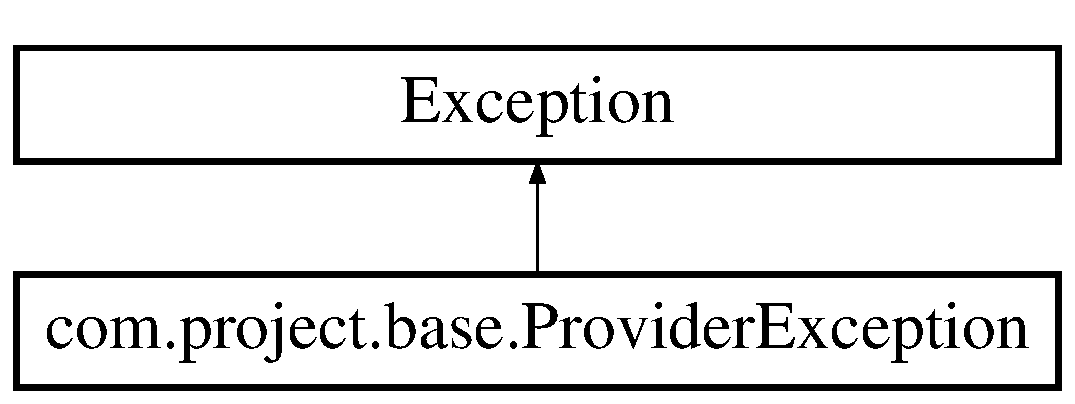
\includegraphics[height=2.000000cm]{classcom_1_1project_1_1base_1_1_provider_exception}
\end{center}
\end{figure}
\subsection*{Public Member Functions}
\begin{DoxyCompactItemize}
\item 
\mbox{\label{classcom_1_1project_1_1base_1_1_provider_exception_ae9596b49f78bb1f132a797e3e11c8748}} 
{\bfseries Provider\+Exception} (String message)
\end{DoxyCompactItemize}


\subsection{Detailed Description}
\begin{DoxyAuthor}{Author}
seweryn 
\end{DoxyAuthor}


The documentation for this class was generated from the following file\+:\begin{DoxyCompactItemize}
\item 
/\+Users/seweryn/\+Net\+Beans\+Projects/\+Ceneo\+H\+D/\+Ceneo\+H\+D-\/lib/src/com/project/base/Provider\+Exception.\+java\end{DoxyCompactItemize}

\section{com.\+project.\+dto.\+Review\+D\+TO Class Reference}
\label{classcom_1_1project_1_1dto_1_1_review_d_t_o}\index{com.\+project.\+dto.\+Review\+D\+TO@{com.\+project.\+dto.\+Review\+D\+TO}}
\subsection*{Public Member Functions}
\begin{DoxyCompactItemize}
\item 
\textbf{ Review\+D\+TO} (String remote\+Id)
\item 
String \textbf{ get\+Remote\+Id} ()
\item 
String \textbf{ get\+Advantages} ()
\item 
void \textbf{ set\+Advantages} (String advantages)
\item 
String \textbf{ get\+Disadvantages} ()
\item 
void \textbf{ set\+Disadvantages} (String disadvantages)
\item 
String \textbf{ get\+Summary} ()
\item 
void \textbf{ set\+Summary} (String summary)
\item 
String \textbf{ get\+Score} ()
\item 
void \textbf{ set\+Score} (String score)
\item 
String \textbf{ get\+Author} ()
\item 
void \textbf{ set\+Author} (String author)
\item 
Date \textbf{ get\+Create\+Date} ()
\item 
void \textbf{ set\+Create\+Date} (Date create\+Date)
\item 
Boolean \textbf{ get\+Is\+Recomended} ()
\item 
void \textbf{ set\+Is\+Recomended} (Boolean is\+Recomended)
\item 
int \textbf{ get\+Likes\+Count} ()
\item 
void \textbf{ set\+Likes\+Count} (int likes\+Count)
\item 
int \textbf{ get\+Dislikes\+Count} ()
\item 
void \textbf{ set\+Dislikes\+Count} (int dislikes\+Count)
\end{DoxyCompactItemize}


\subsection{Detailed Description}
\begin{DoxyAuthor}{Author}
seweryn
\end{DoxyAuthor}
Struktura D\+TO przechowująca dane opini. 

\subsection{Constructor \& Destructor Documentation}
\mbox{\label{classcom_1_1project_1_1dto_1_1_review_d_t_o_a8866367cad594185695184cc5aea0192}} 
\index{com\+::project\+::dto\+::\+Review\+D\+TO@{com\+::project\+::dto\+::\+Review\+D\+TO}!Review\+D\+TO@{Review\+D\+TO}}
\index{Review\+D\+TO@{Review\+D\+TO}!com\+::project\+::dto\+::\+Review\+D\+TO@{com\+::project\+::dto\+::\+Review\+D\+TO}}
\subsubsection{Review\+D\+T\+O()}
{\footnotesize\ttfamily com.\+project.\+dto.\+Review\+D\+T\+O.\+Review\+D\+TO (\begin{DoxyParamCaption}\item[{String}]{remote\+Id }\end{DoxyParamCaption})}


\begin{DoxyParams}{Parameters}
{\em remote\+Id} & zdalne id opini \\
\hline
\end{DoxyParams}


\subsection{Member Function Documentation}
\mbox{\label{classcom_1_1project_1_1dto_1_1_review_d_t_o_a309a1140c9b1ee497a471ea6fd360e7d}} 
\index{com\+::project\+::dto\+::\+Review\+D\+TO@{com\+::project\+::dto\+::\+Review\+D\+TO}!get\+Advantages@{get\+Advantages}}
\index{get\+Advantages@{get\+Advantages}!com\+::project\+::dto\+::\+Review\+D\+TO@{com\+::project\+::dto\+::\+Review\+D\+TO}}
\subsubsection{get\+Advantages()}
{\footnotesize\ttfamily String com.\+project.\+dto.\+Review\+D\+T\+O.\+get\+Advantages (\begin{DoxyParamCaption}{ }\end{DoxyParamCaption})}

\begin{DoxyReturn}{Returns}
the advantages 
\end{DoxyReturn}
\mbox{\label{classcom_1_1project_1_1dto_1_1_review_d_t_o_a79361ce2497daf47a78d0711383fe21a}} 
\index{com\+::project\+::dto\+::\+Review\+D\+TO@{com\+::project\+::dto\+::\+Review\+D\+TO}!get\+Author@{get\+Author}}
\index{get\+Author@{get\+Author}!com\+::project\+::dto\+::\+Review\+D\+TO@{com\+::project\+::dto\+::\+Review\+D\+TO}}
\subsubsection{get\+Author()}
{\footnotesize\ttfamily String com.\+project.\+dto.\+Review\+D\+T\+O.\+get\+Author (\begin{DoxyParamCaption}{ }\end{DoxyParamCaption})}

\begin{DoxyReturn}{Returns}
the author 
\end{DoxyReturn}
\mbox{\label{classcom_1_1project_1_1dto_1_1_review_d_t_o_aa5f70ef29a16c6a4634e3a2400b12582}} 
\index{com\+::project\+::dto\+::\+Review\+D\+TO@{com\+::project\+::dto\+::\+Review\+D\+TO}!get\+Create\+Date@{get\+Create\+Date}}
\index{get\+Create\+Date@{get\+Create\+Date}!com\+::project\+::dto\+::\+Review\+D\+TO@{com\+::project\+::dto\+::\+Review\+D\+TO}}
\subsubsection{get\+Create\+Date()}
{\footnotesize\ttfamily Date com.\+project.\+dto.\+Review\+D\+T\+O.\+get\+Create\+Date (\begin{DoxyParamCaption}{ }\end{DoxyParamCaption})}

\begin{DoxyReturn}{Returns}
the create\+Date 
\end{DoxyReturn}
\mbox{\label{classcom_1_1project_1_1dto_1_1_review_d_t_o_a5502746fafafdde119451e784d8724c5}} 
\index{com\+::project\+::dto\+::\+Review\+D\+TO@{com\+::project\+::dto\+::\+Review\+D\+TO}!get\+Disadvantages@{get\+Disadvantages}}
\index{get\+Disadvantages@{get\+Disadvantages}!com\+::project\+::dto\+::\+Review\+D\+TO@{com\+::project\+::dto\+::\+Review\+D\+TO}}
\subsubsection{get\+Disadvantages()}
{\footnotesize\ttfamily String com.\+project.\+dto.\+Review\+D\+T\+O.\+get\+Disadvantages (\begin{DoxyParamCaption}{ }\end{DoxyParamCaption})}

\begin{DoxyReturn}{Returns}
the disadvantages 
\end{DoxyReturn}
\mbox{\label{classcom_1_1project_1_1dto_1_1_review_d_t_o_a3db59bc3141de3e8652c039c9c47fd0f}} 
\index{com\+::project\+::dto\+::\+Review\+D\+TO@{com\+::project\+::dto\+::\+Review\+D\+TO}!get\+Dislikes\+Count@{get\+Dislikes\+Count}}
\index{get\+Dislikes\+Count@{get\+Dislikes\+Count}!com\+::project\+::dto\+::\+Review\+D\+TO@{com\+::project\+::dto\+::\+Review\+D\+TO}}
\subsubsection{get\+Dislikes\+Count()}
{\footnotesize\ttfamily int com.\+project.\+dto.\+Review\+D\+T\+O.\+get\+Dislikes\+Count (\begin{DoxyParamCaption}{ }\end{DoxyParamCaption})}

\begin{DoxyReturn}{Returns}
the dislikes\+Count 
\end{DoxyReturn}
\mbox{\label{classcom_1_1project_1_1dto_1_1_review_d_t_o_afce41cc3fa88731b17d89b73673e2ccb}} 
\index{com\+::project\+::dto\+::\+Review\+D\+TO@{com\+::project\+::dto\+::\+Review\+D\+TO}!get\+Is\+Recomended@{get\+Is\+Recomended}}
\index{get\+Is\+Recomended@{get\+Is\+Recomended}!com\+::project\+::dto\+::\+Review\+D\+TO@{com\+::project\+::dto\+::\+Review\+D\+TO}}
\subsubsection{get\+Is\+Recomended()}
{\footnotesize\ttfamily Boolean com.\+project.\+dto.\+Review\+D\+T\+O.\+get\+Is\+Recomended (\begin{DoxyParamCaption}{ }\end{DoxyParamCaption})}

\begin{DoxyReturn}{Returns}
the is\+Recomended 
\end{DoxyReturn}
\mbox{\label{classcom_1_1project_1_1dto_1_1_review_d_t_o_aab973053d931109f3f104380ef5ee092}} 
\index{com\+::project\+::dto\+::\+Review\+D\+TO@{com\+::project\+::dto\+::\+Review\+D\+TO}!get\+Likes\+Count@{get\+Likes\+Count}}
\index{get\+Likes\+Count@{get\+Likes\+Count}!com\+::project\+::dto\+::\+Review\+D\+TO@{com\+::project\+::dto\+::\+Review\+D\+TO}}
\subsubsection{get\+Likes\+Count()}
{\footnotesize\ttfamily int com.\+project.\+dto.\+Review\+D\+T\+O.\+get\+Likes\+Count (\begin{DoxyParamCaption}{ }\end{DoxyParamCaption})}

\begin{DoxyReturn}{Returns}
the likes\+Count 
\end{DoxyReturn}
\mbox{\label{classcom_1_1project_1_1dto_1_1_review_d_t_o_a0ea4b143d749f6902b7353e75411a77f}} 
\index{com\+::project\+::dto\+::\+Review\+D\+TO@{com\+::project\+::dto\+::\+Review\+D\+TO}!get\+Remote\+Id@{get\+Remote\+Id}}
\index{get\+Remote\+Id@{get\+Remote\+Id}!com\+::project\+::dto\+::\+Review\+D\+TO@{com\+::project\+::dto\+::\+Review\+D\+TO}}
\subsubsection{get\+Remote\+Id()}
{\footnotesize\ttfamily String com.\+project.\+dto.\+Review\+D\+T\+O.\+get\+Remote\+Id (\begin{DoxyParamCaption}{ }\end{DoxyParamCaption})}

\begin{DoxyReturn}{Returns}
zdalne id opini 
\end{DoxyReturn}
\mbox{\label{classcom_1_1project_1_1dto_1_1_review_d_t_o_ab6709430c27a797db7957fc5b0d1740c}} 
\index{com\+::project\+::dto\+::\+Review\+D\+TO@{com\+::project\+::dto\+::\+Review\+D\+TO}!get\+Score@{get\+Score}}
\index{get\+Score@{get\+Score}!com\+::project\+::dto\+::\+Review\+D\+TO@{com\+::project\+::dto\+::\+Review\+D\+TO}}
\subsubsection{get\+Score()}
{\footnotesize\ttfamily String com.\+project.\+dto.\+Review\+D\+T\+O.\+get\+Score (\begin{DoxyParamCaption}{ }\end{DoxyParamCaption})}

\begin{DoxyReturn}{Returns}
the score 
\end{DoxyReturn}
\mbox{\label{classcom_1_1project_1_1dto_1_1_review_d_t_o_a4a30ca059359854f5f2dab97a6be1bdd}} 
\index{com\+::project\+::dto\+::\+Review\+D\+TO@{com\+::project\+::dto\+::\+Review\+D\+TO}!get\+Summary@{get\+Summary}}
\index{get\+Summary@{get\+Summary}!com\+::project\+::dto\+::\+Review\+D\+TO@{com\+::project\+::dto\+::\+Review\+D\+TO}}
\subsubsection{get\+Summary()}
{\footnotesize\ttfamily String com.\+project.\+dto.\+Review\+D\+T\+O.\+get\+Summary (\begin{DoxyParamCaption}{ }\end{DoxyParamCaption})}

\begin{DoxyReturn}{Returns}
the summary 
\end{DoxyReturn}
\mbox{\label{classcom_1_1project_1_1dto_1_1_review_d_t_o_a0d7851af9a42d2d40c40b2dea2c9ff20}} 
\index{com\+::project\+::dto\+::\+Review\+D\+TO@{com\+::project\+::dto\+::\+Review\+D\+TO}!set\+Advantages@{set\+Advantages}}
\index{set\+Advantages@{set\+Advantages}!com\+::project\+::dto\+::\+Review\+D\+TO@{com\+::project\+::dto\+::\+Review\+D\+TO}}
\subsubsection{set\+Advantages()}
{\footnotesize\ttfamily void com.\+project.\+dto.\+Review\+D\+T\+O.\+set\+Advantages (\begin{DoxyParamCaption}\item[{String}]{advantages }\end{DoxyParamCaption})}


\begin{DoxyParams}{Parameters}
{\em advantages} & the advantages to set \\
\hline
\end{DoxyParams}
\mbox{\label{classcom_1_1project_1_1dto_1_1_review_d_t_o_ae32048e99304608f13d68900900032cd}} 
\index{com\+::project\+::dto\+::\+Review\+D\+TO@{com\+::project\+::dto\+::\+Review\+D\+TO}!set\+Author@{set\+Author}}
\index{set\+Author@{set\+Author}!com\+::project\+::dto\+::\+Review\+D\+TO@{com\+::project\+::dto\+::\+Review\+D\+TO}}
\subsubsection{set\+Author()}
{\footnotesize\ttfamily void com.\+project.\+dto.\+Review\+D\+T\+O.\+set\+Author (\begin{DoxyParamCaption}\item[{String}]{author }\end{DoxyParamCaption})}


\begin{DoxyParams}{Parameters}
{\em author} & the author to set \\
\hline
\end{DoxyParams}
\mbox{\label{classcom_1_1project_1_1dto_1_1_review_d_t_o_a207fc01c87c4b145693a9728023330be}} 
\index{com\+::project\+::dto\+::\+Review\+D\+TO@{com\+::project\+::dto\+::\+Review\+D\+TO}!set\+Create\+Date@{set\+Create\+Date}}
\index{set\+Create\+Date@{set\+Create\+Date}!com\+::project\+::dto\+::\+Review\+D\+TO@{com\+::project\+::dto\+::\+Review\+D\+TO}}
\subsubsection{set\+Create\+Date()}
{\footnotesize\ttfamily void com.\+project.\+dto.\+Review\+D\+T\+O.\+set\+Create\+Date (\begin{DoxyParamCaption}\item[{Date}]{create\+Date }\end{DoxyParamCaption})}


\begin{DoxyParams}{Parameters}
{\em create\+Date} & the create\+Date to set \\
\hline
\end{DoxyParams}
\mbox{\label{classcom_1_1project_1_1dto_1_1_review_d_t_o_abc930abc1fd7c8ff2e2fec2d144efb5b}} 
\index{com\+::project\+::dto\+::\+Review\+D\+TO@{com\+::project\+::dto\+::\+Review\+D\+TO}!set\+Disadvantages@{set\+Disadvantages}}
\index{set\+Disadvantages@{set\+Disadvantages}!com\+::project\+::dto\+::\+Review\+D\+TO@{com\+::project\+::dto\+::\+Review\+D\+TO}}
\subsubsection{set\+Disadvantages()}
{\footnotesize\ttfamily void com.\+project.\+dto.\+Review\+D\+T\+O.\+set\+Disadvantages (\begin{DoxyParamCaption}\item[{String}]{disadvantages }\end{DoxyParamCaption})}


\begin{DoxyParams}{Parameters}
{\em disadvantages} & the disadvantages to set \\
\hline
\end{DoxyParams}
\mbox{\label{classcom_1_1project_1_1dto_1_1_review_d_t_o_a77d5a4733a7450649d5d8a632dc94da3}} 
\index{com\+::project\+::dto\+::\+Review\+D\+TO@{com\+::project\+::dto\+::\+Review\+D\+TO}!set\+Dislikes\+Count@{set\+Dislikes\+Count}}
\index{set\+Dislikes\+Count@{set\+Dislikes\+Count}!com\+::project\+::dto\+::\+Review\+D\+TO@{com\+::project\+::dto\+::\+Review\+D\+TO}}
\subsubsection{set\+Dislikes\+Count()}
{\footnotesize\ttfamily void com.\+project.\+dto.\+Review\+D\+T\+O.\+set\+Dislikes\+Count (\begin{DoxyParamCaption}\item[{int}]{dislikes\+Count }\end{DoxyParamCaption})}


\begin{DoxyParams}{Parameters}
{\em dislikes\+Count} & the dislikes\+Count to set \\
\hline
\end{DoxyParams}
\mbox{\label{classcom_1_1project_1_1dto_1_1_review_d_t_o_ab33c3e31c4847d30ae386ea72c520b1b}} 
\index{com\+::project\+::dto\+::\+Review\+D\+TO@{com\+::project\+::dto\+::\+Review\+D\+TO}!set\+Is\+Recomended@{set\+Is\+Recomended}}
\index{set\+Is\+Recomended@{set\+Is\+Recomended}!com\+::project\+::dto\+::\+Review\+D\+TO@{com\+::project\+::dto\+::\+Review\+D\+TO}}
\subsubsection{set\+Is\+Recomended()}
{\footnotesize\ttfamily void com.\+project.\+dto.\+Review\+D\+T\+O.\+set\+Is\+Recomended (\begin{DoxyParamCaption}\item[{Boolean}]{is\+Recomended }\end{DoxyParamCaption})}


\begin{DoxyParams}{Parameters}
{\em is\+Recomended} & the is\+Recomended to set \\
\hline
\end{DoxyParams}
\mbox{\label{classcom_1_1project_1_1dto_1_1_review_d_t_o_a8b794c0b7c71802b410d4ea881a7b58c}} 
\index{com\+::project\+::dto\+::\+Review\+D\+TO@{com\+::project\+::dto\+::\+Review\+D\+TO}!set\+Likes\+Count@{set\+Likes\+Count}}
\index{set\+Likes\+Count@{set\+Likes\+Count}!com\+::project\+::dto\+::\+Review\+D\+TO@{com\+::project\+::dto\+::\+Review\+D\+TO}}
\subsubsection{set\+Likes\+Count()}
{\footnotesize\ttfamily void com.\+project.\+dto.\+Review\+D\+T\+O.\+set\+Likes\+Count (\begin{DoxyParamCaption}\item[{int}]{likes\+Count }\end{DoxyParamCaption})}


\begin{DoxyParams}{Parameters}
{\em likes\+Count} & the likes\+Count to set \\
\hline
\end{DoxyParams}
\mbox{\label{classcom_1_1project_1_1dto_1_1_review_d_t_o_ac5cab37e8ef89a1820fd649cdc5344e8}} 
\index{com\+::project\+::dto\+::\+Review\+D\+TO@{com\+::project\+::dto\+::\+Review\+D\+TO}!set\+Score@{set\+Score}}
\index{set\+Score@{set\+Score}!com\+::project\+::dto\+::\+Review\+D\+TO@{com\+::project\+::dto\+::\+Review\+D\+TO}}
\subsubsection{set\+Score()}
{\footnotesize\ttfamily void com.\+project.\+dto.\+Review\+D\+T\+O.\+set\+Score (\begin{DoxyParamCaption}\item[{String}]{score }\end{DoxyParamCaption})}


\begin{DoxyParams}{Parameters}
{\em score} & the score to set \\
\hline
\end{DoxyParams}
\mbox{\label{classcom_1_1project_1_1dto_1_1_review_d_t_o_a162e777da302c2fb3dc5a7885471232f}} 
\index{com\+::project\+::dto\+::\+Review\+D\+TO@{com\+::project\+::dto\+::\+Review\+D\+TO}!set\+Summary@{set\+Summary}}
\index{set\+Summary@{set\+Summary}!com\+::project\+::dto\+::\+Review\+D\+TO@{com\+::project\+::dto\+::\+Review\+D\+TO}}
\subsubsection{set\+Summary()}
{\footnotesize\ttfamily void com.\+project.\+dto.\+Review\+D\+T\+O.\+set\+Summary (\begin{DoxyParamCaption}\item[{String}]{summary }\end{DoxyParamCaption})}


\begin{DoxyParams}{Parameters}
{\em summary} & the summary to set \\
\hline
\end{DoxyParams}


The documentation for this class was generated from the following file\+:\begin{DoxyCompactItemize}
\item 
/\+Users/seweryn/\+Net\+Beans\+Projects/\+Ceneo\+H\+D/\+Ceneo\+H\+D-\/lib/src/com/project/dto/Review\+D\+T\+O.\+java\end{DoxyCompactItemize}

\section{com.\+project.\+entity.\+Review\+Entity Class Reference}
\label{classcom_1_1project_1_1entity_1_1_review_entity}\index{com.\+project.\+entity.\+Review\+Entity@{com.\+project.\+entity.\+Review\+Entity}}
\subsection*{Public Member Functions}
\begin{DoxyCompactItemize}
\item 
\textbf{ Review\+Entity} ()
\item 
\textbf{ Review\+Entity} (String remote\+Id, String advantages, String disadvantages, String summary, String score, String author, Date create\+Date, Boolean is\+Recomended, int likes\+Count, int dislikes\+Count)
\item 
Long \textbf{ get\+Id} ()
\item 
String \textbf{ get\+Remote\+Id} ()
\item 
void \textbf{ set\+Product} (\textbf{ Product\+Entity} product)
\item 
\textbf{ Product\+Entity} \textbf{ get\+Product} ()
\item 
String \textbf{ get\+Advantages} ()
\item 
void \textbf{ set\+Advantages} (String advantages)
\item 
String \textbf{ get\+Disadvantages} ()
\item 
void \textbf{ set\+Disadvantages} (String disadvantages)
\item 
String \textbf{ get\+Summary} ()
\item 
void \textbf{ set\+Summary} (String summary)
\item 
String \textbf{ get\+Score} ()
\item 
void \textbf{ set\+Score} (String score)
\item 
String \textbf{ get\+Author} ()
\item 
void \textbf{ set\+Author} (String author)
\item 
Date \textbf{ get\+Create\+Date} ()
\item 
void \textbf{ set\+Create\+Date} (Date create\+Date)
\item 
Boolean \textbf{ get\+Is\+Recomended} ()
\item 
void \textbf{ set\+Is\+Recomended} (Boolean is\+Recomended)
\item 
int \textbf{ get\+Likes\+Count} ()
\item 
void \textbf{ set\+Likes\+Count} (int likes\+Count)
\item 
int \textbf{ get\+Dislikes\+Count} ()
\item 
void \textbf{ set\+Dislikes\+Count} (int dislikes\+Count)
\end{DoxyCompactItemize}


\subsection{Detailed Description}
\begin{DoxyAuthor}{Author}
seweryn
\end{DoxyAuthor}
Encja definiująca tabelę produktów w bazie danych. 

\subsection{Constructor \& Destructor Documentation}
\mbox{\label{classcom_1_1project_1_1entity_1_1_review_entity_aa6e9799a82a57959832038606fa3f8d0}} 
\index{com\+::project\+::entity\+::\+Review\+Entity@{com\+::project\+::entity\+::\+Review\+Entity}!Review\+Entity@{Review\+Entity}}
\index{Review\+Entity@{Review\+Entity}!com\+::project\+::entity\+::\+Review\+Entity@{com\+::project\+::entity\+::\+Review\+Entity}}
\subsubsection{Review\+Entity()\hspace{0.1cm}{\footnotesize\ttfamily [1/2]}}
{\footnotesize\ttfamily com.\+project.\+entity.\+Review\+Entity.\+Review\+Entity (\begin{DoxyParamCaption}{ }\end{DoxyParamCaption})}

Konstruktor domyślny \mbox{\label{classcom_1_1project_1_1entity_1_1_review_entity_a2252f104aeda2d5b7c0d39b72490984e}} 
\index{com\+::project\+::entity\+::\+Review\+Entity@{com\+::project\+::entity\+::\+Review\+Entity}!Review\+Entity@{Review\+Entity}}
\index{Review\+Entity@{Review\+Entity}!com\+::project\+::entity\+::\+Review\+Entity@{com\+::project\+::entity\+::\+Review\+Entity}}
\subsubsection{Review\+Entity()\hspace{0.1cm}{\footnotesize\ttfamily [2/2]}}
{\footnotesize\ttfamily com.\+project.\+entity.\+Review\+Entity.\+Review\+Entity (\begin{DoxyParamCaption}\item[{String}]{remote\+Id,  }\item[{String}]{advantages,  }\item[{String}]{disadvantages,  }\item[{String}]{summary,  }\item[{String}]{score,  }\item[{String}]{author,  }\item[{Date}]{create\+Date,  }\item[{Boolean}]{is\+Recomended,  }\item[{int}]{likes\+Count,  }\item[{int}]{dislikes\+Count }\end{DoxyParamCaption})}


\begin{DoxyParams}{Parameters}
{\em remote\+Id} & \\
\hline
{\em advantages} & \\
\hline
{\em disadvantages} & \\
\hline
{\em summary} & \\
\hline
{\em score} & \\
\hline
{\em author} & \\
\hline
{\em create\+Date} & \\
\hline
{\em is\+Recomended} & \\
\hline
{\em likes\+Count} & \\
\hline
{\em dislikes\+Count} & \\
\hline
\end{DoxyParams}


\subsection{Member Function Documentation}
\mbox{\label{classcom_1_1project_1_1entity_1_1_review_entity_acfed6d4489b344fcce955b3fbbf8af4c}} 
\index{com\+::project\+::entity\+::\+Review\+Entity@{com\+::project\+::entity\+::\+Review\+Entity}!get\+Advantages@{get\+Advantages}}
\index{get\+Advantages@{get\+Advantages}!com\+::project\+::entity\+::\+Review\+Entity@{com\+::project\+::entity\+::\+Review\+Entity}}
\subsubsection{get\+Advantages()}
{\footnotesize\ttfamily String com.\+project.\+entity.\+Review\+Entity.\+get\+Advantages (\begin{DoxyParamCaption}{ }\end{DoxyParamCaption})}

\begin{DoxyReturn}{Returns}
the advantages 
\end{DoxyReturn}
\mbox{\label{classcom_1_1project_1_1entity_1_1_review_entity_aefc275687e4ecdb029509d88ab4c4a4e}} 
\index{com\+::project\+::entity\+::\+Review\+Entity@{com\+::project\+::entity\+::\+Review\+Entity}!get\+Author@{get\+Author}}
\index{get\+Author@{get\+Author}!com\+::project\+::entity\+::\+Review\+Entity@{com\+::project\+::entity\+::\+Review\+Entity}}
\subsubsection{get\+Author()}
{\footnotesize\ttfamily String com.\+project.\+entity.\+Review\+Entity.\+get\+Author (\begin{DoxyParamCaption}{ }\end{DoxyParamCaption})}

\begin{DoxyReturn}{Returns}
the author 
\end{DoxyReturn}
\mbox{\label{classcom_1_1project_1_1entity_1_1_review_entity_a4ed94879a4aa57ddbd4b2278308290fd}} 
\index{com\+::project\+::entity\+::\+Review\+Entity@{com\+::project\+::entity\+::\+Review\+Entity}!get\+Create\+Date@{get\+Create\+Date}}
\index{get\+Create\+Date@{get\+Create\+Date}!com\+::project\+::entity\+::\+Review\+Entity@{com\+::project\+::entity\+::\+Review\+Entity}}
\subsubsection{get\+Create\+Date()}
{\footnotesize\ttfamily Date com.\+project.\+entity.\+Review\+Entity.\+get\+Create\+Date (\begin{DoxyParamCaption}{ }\end{DoxyParamCaption})}

\begin{DoxyReturn}{Returns}
the create\+Date 
\end{DoxyReturn}
\mbox{\label{classcom_1_1project_1_1entity_1_1_review_entity_a0cefe0b14a6e2ca3071e4d8f8d808d74}} 
\index{com\+::project\+::entity\+::\+Review\+Entity@{com\+::project\+::entity\+::\+Review\+Entity}!get\+Disadvantages@{get\+Disadvantages}}
\index{get\+Disadvantages@{get\+Disadvantages}!com\+::project\+::entity\+::\+Review\+Entity@{com\+::project\+::entity\+::\+Review\+Entity}}
\subsubsection{get\+Disadvantages()}
{\footnotesize\ttfamily String com.\+project.\+entity.\+Review\+Entity.\+get\+Disadvantages (\begin{DoxyParamCaption}{ }\end{DoxyParamCaption})}

\begin{DoxyReturn}{Returns}
the disadvantages 
\end{DoxyReturn}
\mbox{\label{classcom_1_1project_1_1entity_1_1_review_entity_a305a3232fefb4170d05265da012cd7d4}} 
\index{com\+::project\+::entity\+::\+Review\+Entity@{com\+::project\+::entity\+::\+Review\+Entity}!get\+Dislikes\+Count@{get\+Dislikes\+Count}}
\index{get\+Dislikes\+Count@{get\+Dislikes\+Count}!com\+::project\+::entity\+::\+Review\+Entity@{com\+::project\+::entity\+::\+Review\+Entity}}
\subsubsection{get\+Dislikes\+Count()}
{\footnotesize\ttfamily int com.\+project.\+entity.\+Review\+Entity.\+get\+Dislikes\+Count (\begin{DoxyParamCaption}{ }\end{DoxyParamCaption})}

\begin{DoxyReturn}{Returns}
the dislikes\+Count 
\end{DoxyReturn}
\mbox{\label{classcom_1_1project_1_1entity_1_1_review_entity_a70b3c05e52e5294c2bc80d75669f62f1}} 
\index{com\+::project\+::entity\+::\+Review\+Entity@{com\+::project\+::entity\+::\+Review\+Entity}!get\+Id@{get\+Id}}
\index{get\+Id@{get\+Id}!com\+::project\+::entity\+::\+Review\+Entity@{com\+::project\+::entity\+::\+Review\+Entity}}
\subsubsection{get\+Id()}
{\footnotesize\ttfamily Long com.\+project.\+entity.\+Review\+Entity.\+get\+Id (\begin{DoxyParamCaption}{ }\end{DoxyParamCaption})}

\begin{DoxyReturn}{Returns}
id 
\end{DoxyReturn}
\mbox{\label{classcom_1_1project_1_1entity_1_1_review_entity_a174454ada463f86ac8ad6ba374c796c4}} 
\index{com\+::project\+::entity\+::\+Review\+Entity@{com\+::project\+::entity\+::\+Review\+Entity}!get\+Is\+Recomended@{get\+Is\+Recomended}}
\index{get\+Is\+Recomended@{get\+Is\+Recomended}!com\+::project\+::entity\+::\+Review\+Entity@{com\+::project\+::entity\+::\+Review\+Entity}}
\subsubsection{get\+Is\+Recomended()}
{\footnotesize\ttfamily Boolean com.\+project.\+entity.\+Review\+Entity.\+get\+Is\+Recomended (\begin{DoxyParamCaption}{ }\end{DoxyParamCaption})}

\begin{DoxyReturn}{Returns}
the is\+Recomended 
\end{DoxyReturn}
\mbox{\label{classcom_1_1project_1_1entity_1_1_review_entity_afee35f1856c2602eade45a88b30f8f4c}} 
\index{com\+::project\+::entity\+::\+Review\+Entity@{com\+::project\+::entity\+::\+Review\+Entity}!get\+Likes\+Count@{get\+Likes\+Count}}
\index{get\+Likes\+Count@{get\+Likes\+Count}!com\+::project\+::entity\+::\+Review\+Entity@{com\+::project\+::entity\+::\+Review\+Entity}}
\subsubsection{get\+Likes\+Count()}
{\footnotesize\ttfamily int com.\+project.\+entity.\+Review\+Entity.\+get\+Likes\+Count (\begin{DoxyParamCaption}{ }\end{DoxyParamCaption})}

\begin{DoxyReturn}{Returns}
the likes\+Count 
\end{DoxyReturn}
\mbox{\label{classcom_1_1project_1_1entity_1_1_review_entity_a3823beaab4a7d3edf9d35ebe77d8daee}} 
\index{com\+::project\+::entity\+::\+Review\+Entity@{com\+::project\+::entity\+::\+Review\+Entity}!get\+Product@{get\+Product}}
\index{get\+Product@{get\+Product}!com\+::project\+::entity\+::\+Review\+Entity@{com\+::project\+::entity\+::\+Review\+Entity}}
\subsubsection{get\+Product()}
{\footnotesize\ttfamily \textbf{ Product\+Entity} com.\+project.\+entity.\+Review\+Entity.\+get\+Product (\begin{DoxyParamCaption}{ }\end{DoxyParamCaption})}

\begin{DoxyReturn}{Returns}
product\+Entity 
\end{DoxyReturn}
\mbox{\label{classcom_1_1project_1_1entity_1_1_review_entity_afedba077d5835d7b914d4672f199a83e}} 
\index{com\+::project\+::entity\+::\+Review\+Entity@{com\+::project\+::entity\+::\+Review\+Entity}!get\+Remote\+Id@{get\+Remote\+Id}}
\index{get\+Remote\+Id@{get\+Remote\+Id}!com\+::project\+::entity\+::\+Review\+Entity@{com\+::project\+::entity\+::\+Review\+Entity}}
\subsubsection{get\+Remote\+Id()}
{\footnotesize\ttfamily String com.\+project.\+entity.\+Review\+Entity.\+get\+Remote\+Id (\begin{DoxyParamCaption}{ }\end{DoxyParamCaption})}

\begin{DoxyReturn}{Returns}
remote\+Id 
\end{DoxyReturn}
\mbox{\label{classcom_1_1project_1_1entity_1_1_review_entity_ab33fd76de384b57fbb2276683f6e1a0c}} 
\index{com\+::project\+::entity\+::\+Review\+Entity@{com\+::project\+::entity\+::\+Review\+Entity}!get\+Score@{get\+Score}}
\index{get\+Score@{get\+Score}!com\+::project\+::entity\+::\+Review\+Entity@{com\+::project\+::entity\+::\+Review\+Entity}}
\subsubsection{get\+Score()}
{\footnotesize\ttfamily String com.\+project.\+entity.\+Review\+Entity.\+get\+Score (\begin{DoxyParamCaption}{ }\end{DoxyParamCaption})}

\begin{DoxyReturn}{Returns}
the score 
\end{DoxyReturn}
\mbox{\label{classcom_1_1project_1_1entity_1_1_review_entity_a5a9fd2b78dcbd2f34e2d73effebbf45d}} 
\index{com\+::project\+::entity\+::\+Review\+Entity@{com\+::project\+::entity\+::\+Review\+Entity}!get\+Summary@{get\+Summary}}
\index{get\+Summary@{get\+Summary}!com\+::project\+::entity\+::\+Review\+Entity@{com\+::project\+::entity\+::\+Review\+Entity}}
\subsubsection{get\+Summary()}
{\footnotesize\ttfamily String com.\+project.\+entity.\+Review\+Entity.\+get\+Summary (\begin{DoxyParamCaption}{ }\end{DoxyParamCaption})}

\begin{DoxyReturn}{Returns}
the summary 
\end{DoxyReturn}
\mbox{\label{classcom_1_1project_1_1entity_1_1_review_entity_a96442854e8c7a0bc020f6abe29d9a2d6}} 
\index{com\+::project\+::entity\+::\+Review\+Entity@{com\+::project\+::entity\+::\+Review\+Entity}!set\+Advantages@{set\+Advantages}}
\index{set\+Advantages@{set\+Advantages}!com\+::project\+::entity\+::\+Review\+Entity@{com\+::project\+::entity\+::\+Review\+Entity}}
\subsubsection{set\+Advantages()}
{\footnotesize\ttfamily void com.\+project.\+entity.\+Review\+Entity.\+set\+Advantages (\begin{DoxyParamCaption}\item[{String}]{advantages }\end{DoxyParamCaption})}


\begin{DoxyParams}{Parameters}
{\em advantages} & the advantages to set \\
\hline
\end{DoxyParams}
\mbox{\label{classcom_1_1project_1_1entity_1_1_review_entity_acd3b24891ec352f74a30acb7ad0a0d00}} 
\index{com\+::project\+::entity\+::\+Review\+Entity@{com\+::project\+::entity\+::\+Review\+Entity}!set\+Author@{set\+Author}}
\index{set\+Author@{set\+Author}!com\+::project\+::entity\+::\+Review\+Entity@{com\+::project\+::entity\+::\+Review\+Entity}}
\subsubsection{set\+Author()}
{\footnotesize\ttfamily void com.\+project.\+entity.\+Review\+Entity.\+set\+Author (\begin{DoxyParamCaption}\item[{String}]{author }\end{DoxyParamCaption})}


\begin{DoxyParams}{Parameters}
{\em author} & the author to set \\
\hline
\end{DoxyParams}
\mbox{\label{classcom_1_1project_1_1entity_1_1_review_entity_a8334754619b1add923c6219d5e80bf9c}} 
\index{com\+::project\+::entity\+::\+Review\+Entity@{com\+::project\+::entity\+::\+Review\+Entity}!set\+Create\+Date@{set\+Create\+Date}}
\index{set\+Create\+Date@{set\+Create\+Date}!com\+::project\+::entity\+::\+Review\+Entity@{com\+::project\+::entity\+::\+Review\+Entity}}
\subsubsection{set\+Create\+Date()}
{\footnotesize\ttfamily void com.\+project.\+entity.\+Review\+Entity.\+set\+Create\+Date (\begin{DoxyParamCaption}\item[{Date}]{create\+Date }\end{DoxyParamCaption})}


\begin{DoxyParams}{Parameters}
{\em create\+Date} & the create\+Date to set \\
\hline
\end{DoxyParams}
\mbox{\label{classcom_1_1project_1_1entity_1_1_review_entity_adb038f1842856a3231e791ab74018616}} 
\index{com\+::project\+::entity\+::\+Review\+Entity@{com\+::project\+::entity\+::\+Review\+Entity}!set\+Disadvantages@{set\+Disadvantages}}
\index{set\+Disadvantages@{set\+Disadvantages}!com\+::project\+::entity\+::\+Review\+Entity@{com\+::project\+::entity\+::\+Review\+Entity}}
\subsubsection{set\+Disadvantages()}
{\footnotesize\ttfamily void com.\+project.\+entity.\+Review\+Entity.\+set\+Disadvantages (\begin{DoxyParamCaption}\item[{String}]{disadvantages }\end{DoxyParamCaption})}


\begin{DoxyParams}{Parameters}
{\em disadvantages} & the disadvantages to set \\
\hline
\end{DoxyParams}
\mbox{\label{classcom_1_1project_1_1entity_1_1_review_entity_ae53e12d28656804a5a41666f4439044b}} 
\index{com\+::project\+::entity\+::\+Review\+Entity@{com\+::project\+::entity\+::\+Review\+Entity}!set\+Dislikes\+Count@{set\+Dislikes\+Count}}
\index{set\+Dislikes\+Count@{set\+Dislikes\+Count}!com\+::project\+::entity\+::\+Review\+Entity@{com\+::project\+::entity\+::\+Review\+Entity}}
\subsubsection{set\+Dislikes\+Count()}
{\footnotesize\ttfamily void com.\+project.\+entity.\+Review\+Entity.\+set\+Dislikes\+Count (\begin{DoxyParamCaption}\item[{int}]{dislikes\+Count }\end{DoxyParamCaption})}


\begin{DoxyParams}{Parameters}
{\em dislikes\+Count} & the dislikes\+Count to set \\
\hline
\end{DoxyParams}
\mbox{\label{classcom_1_1project_1_1entity_1_1_review_entity_aee2eace49f40dcad589458cfe376ee16}} 
\index{com\+::project\+::entity\+::\+Review\+Entity@{com\+::project\+::entity\+::\+Review\+Entity}!set\+Is\+Recomended@{set\+Is\+Recomended}}
\index{set\+Is\+Recomended@{set\+Is\+Recomended}!com\+::project\+::entity\+::\+Review\+Entity@{com\+::project\+::entity\+::\+Review\+Entity}}
\subsubsection{set\+Is\+Recomended()}
{\footnotesize\ttfamily void com.\+project.\+entity.\+Review\+Entity.\+set\+Is\+Recomended (\begin{DoxyParamCaption}\item[{Boolean}]{is\+Recomended }\end{DoxyParamCaption})}


\begin{DoxyParams}{Parameters}
{\em is\+Recomended} & the is\+Recomended to set \\
\hline
\end{DoxyParams}
\mbox{\label{classcom_1_1project_1_1entity_1_1_review_entity_abebc1f5fa86f59161240fdb489a27211}} 
\index{com\+::project\+::entity\+::\+Review\+Entity@{com\+::project\+::entity\+::\+Review\+Entity}!set\+Likes\+Count@{set\+Likes\+Count}}
\index{set\+Likes\+Count@{set\+Likes\+Count}!com\+::project\+::entity\+::\+Review\+Entity@{com\+::project\+::entity\+::\+Review\+Entity}}
\subsubsection{set\+Likes\+Count()}
{\footnotesize\ttfamily void com.\+project.\+entity.\+Review\+Entity.\+set\+Likes\+Count (\begin{DoxyParamCaption}\item[{int}]{likes\+Count }\end{DoxyParamCaption})}


\begin{DoxyParams}{Parameters}
{\em likes\+Count} & the likes\+Count to set \\
\hline
\end{DoxyParams}
\mbox{\label{classcom_1_1project_1_1entity_1_1_review_entity_a011433f2e521275e66c54e8027b898aa}} 
\index{com\+::project\+::entity\+::\+Review\+Entity@{com\+::project\+::entity\+::\+Review\+Entity}!set\+Product@{set\+Product}}
\index{set\+Product@{set\+Product}!com\+::project\+::entity\+::\+Review\+Entity@{com\+::project\+::entity\+::\+Review\+Entity}}
\subsubsection{set\+Product()}
{\footnotesize\ttfamily void com.\+project.\+entity.\+Review\+Entity.\+set\+Product (\begin{DoxyParamCaption}\item[{\textbf{ Product\+Entity}}]{product }\end{DoxyParamCaption})}


\begin{DoxyParams}{Parameters}
{\em product} & \\
\hline
\end{DoxyParams}
\mbox{\label{classcom_1_1project_1_1entity_1_1_review_entity_aee6d7c1df3c51fe94ae2353890127cf8}} 
\index{com\+::project\+::entity\+::\+Review\+Entity@{com\+::project\+::entity\+::\+Review\+Entity}!set\+Score@{set\+Score}}
\index{set\+Score@{set\+Score}!com\+::project\+::entity\+::\+Review\+Entity@{com\+::project\+::entity\+::\+Review\+Entity}}
\subsubsection{set\+Score()}
{\footnotesize\ttfamily void com.\+project.\+entity.\+Review\+Entity.\+set\+Score (\begin{DoxyParamCaption}\item[{String}]{score }\end{DoxyParamCaption})}


\begin{DoxyParams}{Parameters}
{\em score} & the score to set \\
\hline
\end{DoxyParams}
\mbox{\label{classcom_1_1project_1_1entity_1_1_review_entity_af87c71a53c39bf128f42792e3a1bd1f6}} 
\index{com\+::project\+::entity\+::\+Review\+Entity@{com\+::project\+::entity\+::\+Review\+Entity}!set\+Summary@{set\+Summary}}
\index{set\+Summary@{set\+Summary}!com\+::project\+::entity\+::\+Review\+Entity@{com\+::project\+::entity\+::\+Review\+Entity}}
\subsubsection{set\+Summary()}
{\footnotesize\ttfamily void com.\+project.\+entity.\+Review\+Entity.\+set\+Summary (\begin{DoxyParamCaption}\item[{String}]{summary }\end{DoxyParamCaption})}


\begin{DoxyParams}{Parameters}
{\em summary} & the summary to set \\
\hline
\end{DoxyParams}


The documentation for this class was generated from the following file\+:\begin{DoxyCompactItemize}
\item 
/\+Users/seweryn/\+Net\+Beans\+Projects/\+Ceneo\+H\+D/\+Ceneo\+H\+D-\/lib/src/com/project/entity/Review\+Entity.\+java\end{DoxyCompactItemize}

\section{com.\+project.\+base.\+Use\+Case$<$ R\+E\+Q\+U\+E\+S\+T\+\_\+\+O\+B\+J\+E\+CT, R\+E\+S\+P\+O\+N\+S\+E\+\_\+\+O\+B\+J\+E\+CT $>$ Interface Template Reference}
\label{interfacecom_1_1project_1_1base_1_1_use_case}\index{com.\+project.\+base.\+Use\+Case$<$ R\+E\+Q\+U\+E\+S\+T\+\_\+\+O\+B\+J\+E\+C\+T, R\+E\+S\+P\+O\+N\+S\+E\+\_\+\+O\+B\+J\+E\+C\+T $>$@{com.\+project.\+base.\+Use\+Case$<$ R\+E\+Q\+U\+E\+S\+T\+\_\+\+O\+B\+J\+E\+C\+T, R\+E\+S\+P\+O\+N\+S\+E\+\_\+\+O\+B\+J\+E\+C\+T $>$}}


Inherited by com.\+project.\+application.\+Clear\+Database\+Use\+Case, com.\+project.\+application.\+E\+T\+L\+Product\+Use\+Case, com.\+project.\+application.\+Export\+Reviews\+Use\+Case, com.\+project.\+application.\+Extract\+Product\+Use\+Case, com.\+project.\+application.\+Initialize\+Application\+Use\+Case, com.\+project.\+application.\+Load\+Products\+Use\+Case, com.\+project.\+application.\+Load\+Reviews\+Use\+Case, com.\+project.\+application.\+Save\+Product\+Use\+Case, com.\+project.\+application.\+Search\+Products\+Use\+Case, and com.\+project.\+application.\+Transform\+Product\+Use\+Case.

\subsection*{Public Member Functions}
\begin{DoxyCompactItemize}
\item 
R\+E\+S\+P\+O\+N\+S\+E\+\_\+\+O\+B\+J\+E\+CT \textbf{ execute} (R\+E\+Q\+U\+E\+S\+T\+\_\+\+O\+B\+J\+E\+CT request)  throws Throwable
\end{DoxyCompactItemize}


\subsection{Detailed Description}
\begin{DoxyAuthor}{Author}
seweryn
\end{DoxyAuthor}
Ten interfejs realizuje wzorzec polecenia. \doxyref{Use\+Case}{p.}{interfacecom_1_1project_1_1base_1_1_use_case} jest obiektem który może wykonać operacje, przyjmując argumentu (R\+E\+Q\+U\+E\+S\+T\+\_\+\+O\+B\+J\+E\+CT) oraz zwracającą wynik (R\+E\+S\+P\+O\+N\+S\+E\+\_\+\+O\+B\+J\+E\+CT). Operacja \doxyref{Use\+Case}{p.}{interfacecom_1_1project_1_1base_1_1_use_case}\textquotesingle{}a zazwyczaj odpowiada za rozwiązanie biznesowego przypadku użycia i jest wywołaniem blokującym. \doxyref{Use\+Case}{p.}{interfacecom_1_1project_1_1base_1_1_use_case} może zostać wykonany bezpośrednio wywołując metodę \doxyref{execute()}{p.}{interfacecom_1_1project_1_1base_1_1_use_case_ae994e67e62f836c4ec9499cef4eb8eef} lub za pomocą \doxyref{Use\+Case\+Executor}{p.}{interfacecom_1_1project_1_1base_1_1_use_case_executor}\textquotesingle{}a.


\begin{DoxyParams}{Parameters}
{\em $<$\+R\+E\+Q\+U\+E\+S\+T\+\_\+\+O\+B\+J\+E\+C\+T$>$} & -\/ typ argumentu operacji \\
\hline
{\em $<$\+R\+E\+S\+P\+O\+N\+S\+E\+\_\+\+O\+B\+J\+E\+C\+T$>$} & -\/ typ wyniku operacji \\
\hline
\end{DoxyParams}


\subsection{Member Function Documentation}
\mbox{\label{interfacecom_1_1project_1_1base_1_1_use_case_ae994e67e62f836c4ec9499cef4eb8eef}} 
\index{com\+::project\+::base\+::\+Use\+Case@{com\+::project\+::base\+::\+Use\+Case}!execute@{execute}}
\index{execute@{execute}!com\+::project\+::base\+::\+Use\+Case@{com\+::project\+::base\+::\+Use\+Case}}
\subsubsection{execute()}
{\footnotesize\ttfamily R\+E\+S\+P\+O\+N\+S\+E\+\_\+\+O\+B\+J\+E\+CT \textbf{ com.\+project.\+base.\+Use\+Case}$<$ R\+E\+Q\+U\+E\+S\+T\+\_\+\+O\+B\+J\+E\+CT, R\+E\+S\+P\+O\+N\+S\+E\+\_\+\+O\+B\+J\+E\+CT $>$.execute (\begin{DoxyParamCaption}\item[{R\+E\+Q\+U\+E\+S\+T\+\_\+\+O\+B\+J\+E\+CT}]{request }\end{DoxyParamCaption}) throws Throwable}


\begin{DoxyParams}{Parameters}
{\em request} & -\/ argument operacji \\
\hline
\end{DoxyParams}
\begin{DoxyReturn}{Returns}
-\/ wynik operacji 
\end{DoxyReturn}

\begin{DoxyExceptions}{Exceptions}
{\em Throwable} & -\/ błąd zgłoszony podczas wykonania \\
\hline
\end{DoxyExceptions}


The documentation for this interface was generated from the following file\+:\begin{DoxyCompactItemize}
\item 
/\+Users/seweryn/\+Net\+Beans\+Projects/\+Ceneo\+H\+D/\+Ceneo\+H\+D-\/lib/src/com/project/base/Use\+Case.\+java\end{DoxyCompactItemize}

\section{com.\+project.\+base.\+Use\+Case\+Executor Interface Reference}
\label{interfacecom_1_1project_1_1base_1_1_use_case_executor}\index{com.\+project.\+base.\+Use\+Case\+Executor@{com.\+project.\+base.\+Use\+Case\+Executor}}


Inherited by com.\+project.\+application.\+Thread\+Use\+Case\+Executor.

\subsection*{Public Member Functions}
\begin{DoxyCompactItemize}
\item 
$<$ R\+E\+Q\+U\+E\+S\+T\+\_\+\+O\+B\+J\+E\+CT, R\+E\+S\+P\+O\+N\+S\+E\+\_\+\+O\+B\+J\+E\+CT $>$ void \textbf{ execute} (\textbf{ Use\+Case}$<$ R\+E\+Q\+U\+E\+S\+T\+\_\+\+O\+B\+J\+E\+CT, R\+E\+S\+P\+O\+N\+S\+E\+\_\+\+O\+B\+J\+E\+CT $>$ usecase, R\+E\+Q\+U\+E\+S\+T\+\_\+\+O\+B\+J\+E\+CT argument, \textbf{ On\+Success\+Listener}$<$ R\+E\+S\+P\+O\+N\+S\+E\+\_\+\+O\+B\+J\+E\+CT $>$ on\+Success, \textbf{ On\+Error\+Listener} on\+Error)
\end{DoxyCompactItemize}


\subsection{Detailed Description}
\begin{DoxyAuthor}{Author}
seweryn
\end{DoxyAuthor}
Ten interface realizuje wykonanie operacji \doxyref{Use\+Case}{p.}{interfacecom_1_1project_1_1base_1_1_use_case} i obsługuje dostarczenie jej wyniku. Jeśeli operacja wykonania jest przeprowadzana w tle, odpowiedź powinna zostać dostarczona w wątku UI. 

\subsection{Member Function Documentation}
\mbox{\label{interfacecom_1_1project_1_1base_1_1_use_case_executor_aa7bc0e001c7541e5eb846bc987af2e73}} 
\index{com\+::project\+::base\+::\+Use\+Case\+Executor@{com\+::project\+::base\+::\+Use\+Case\+Executor}!execute@{execute}}
\index{execute@{execute}!com\+::project\+::base\+::\+Use\+Case\+Executor@{com\+::project\+::base\+::\+Use\+Case\+Executor}}
\subsubsection{execute()}
{\footnotesize\ttfamily $<$R\+E\+Q\+U\+E\+S\+T\+\_\+\+O\+B\+J\+E\+CT,R\+E\+S\+P\+O\+N\+S\+E\+\_\+\+O\+B\+J\+E\+CT$>$ void com.\+project.\+base.\+Use\+Case\+Executor.\+execute (\begin{DoxyParamCaption}\item[{\textbf{ Use\+Case}$<$ R\+E\+Q\+U\+E\+S\+T\+\_\+\+O\+B\+J\+E\+CT, R\+E\+S\+P\+O\+N\+S\+E\+\_\+\+O\+B\+J\+E\+CT $>$}]{usecase,  }\item[{R\+E\+Q\+U\+E\+S\+T\+\_\+\+O\+B\+J\+E\+CT}]{argument,  }\item[{\textbf{ On\+Success\+Listener}$<$ R\+E\+S\+P\+O\+N\+S\+E\+\_\+\+O\+B\+J\+E\+CT $>$}]{on\+Success,  }\item[{\textbf{ On\+Error\+Listener}}]{on\+Error }\end{DoxyParamCaption})}


\begin{DoxyParams}{Parameters}
{\em $<$\+R\+E\+Q\+U\+E\+S\+T\+\_\+\+O\+B\+J\+E\+C\+T$>$} & -\/ typ argumentu operacji \\
\hline
{\em $<$\+R\+E\+S\+P\+O\+N\+S\+E\+\_\+\+O\+B\+J\+E\+C\+T$>$} & -\/ typ wyniku operacji \\
\hline
{\em usecase} & -\/ \doxyref{Use\+Case}{p.}{interfacecom_1_1project_1_1base_1_1_use_case}, który ma być wykonany \\
\hline
{\em argument} & -\/ argument operacji \\
\hline
{\em on\+Success} & -\/ listener wywołany po wykonaniu operacji \\
\hline
{\em on\+Error} & -\/ listener wywołany w przypadku błędu wykonania \\
\hline
\end{DoxyParams}


The documentation for this interface was generated from the following file\+:\begin{DoxyCompactItemize}
\item 
/\+Users/seweryn/\+Net\+Beans\+Projects/\+Ceneo\+H\+D/\+Ceneo\+H\+D-\/lib/src/com/project/base/Use\+Case\+Executor.\+java\end{DoxyCompactItemize}

%--- End generated contents ---

% Index
\backmatter
\newpage
\phantomsection
\clearemptydoublepage
\addcontentsline{toc}{chapter}{Index}
\printindex

\end{document}
